\documentclass[9pt]{article}
\usepackage[ngerman]{babel}
\usepackage{amsmath,amssymb}
\usepackage[
top=0.5cm,
bottom=2cm,
left=0.5cm,
right=0.5cm
]{geometry}
\usepackage{booktabs}
\usepackage{enumitem}
\usepackage{graphicx}
\usepackage{multicol}
\usepackage{caption}
\usepackage{titlesec}
\usepackage{needspace}
\usepackage{titlesec}

\titleformat{\section}
{\normalfont\normalsize\bfseries}
{\thesection}{2em}{}

\titlespacing*{\section}
{0pt}{1ex}{0.5ex}

% SUBSECTION
\titleformat{\subsection}
{\normalfont\small\bfseries}
{\thesubsection}{1em}{}

\titlespacing*{\subsection}
{0pt}{1.0ex}{0.4ex}


\setlength{\columnsep}{0.6cm}
\setlength{\columnseprule}{0pt}
\raggedcolumns



\begin{document}
    
    \begin{multicols}{2}
        
        \tableofcontents
        
        \section{Grundlagen BWL \& St. Galler Management Modell (SGMM)}
        
        \textbf{BWL:} Lehre von der Planung, Organisation und Kontrolle wirtschaftlicher Aktivitäten in Unternehmen.
        
        \textbf{SGMM – Kernelemente}
        \begin{itemize}[noitemsep]
            \item \textbf{Umweltsphären:} Gesellschaft, Natur, Technologie, Wirtschaft
            \item \textbf{Anspruchsgruppen:} Kunden, Mitarbeitende, Kapitalgeber, Lieferanten, Staat, Öffentlichkeit
            \item \textbf{Prozesse:}
            \begin{itemize}
                \item Managementprozesse
                \item Geschäftsprozesse
                \item Unterstützungsprozesse
            \end{itemize}
            \item \textbf{Ordnungsmomente:} Strategie, Struktur, Kultur
            \item \textbf{Entiwcklungsmodi:} Erneuerung, Optimierung
        \end{itemize}
        \begin{center}
            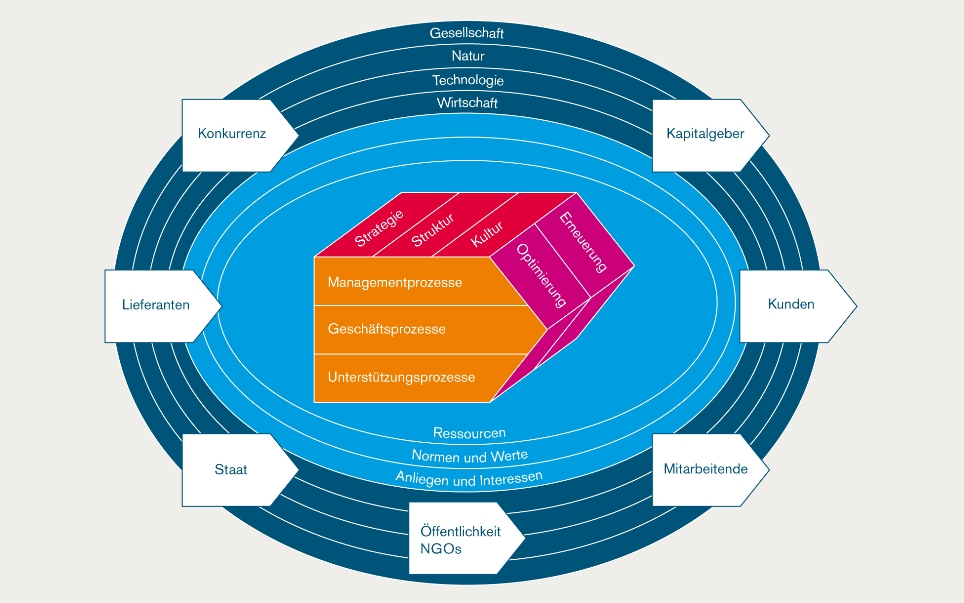
\includegraphics[width=1\linewidth]{./img/sgmm}
            \captionof{figure}{St.Galler Management-Model}
        \end{center}
        
        \section{Strategie}
        
        \textbf{Strategie = langfristiger Weg zur Zielerreichung}
        
        \textbf{Ebenen}
        \begin{itemize}[noitemsep]
            \item \textbf{Normativ:} Vision, Mission, Werte
            \item \textbf{Strategisch:} Wettbewerbsvorteile, Positionierung
            \item \textbf{Operativ:} Umsetzung im Tagesgeschäft
        \end{itemize}
        
        \subsection{Strategische Analyse}
        
        \paragraph{SWOT}
        \[
        \text{Stärken / Schwächen (intern)}, \quad \text{Chancen / Risiken (extern)}
        \]
        
        \paragraph{Porter – 5 Forces}\mbox{}\\
        \begin{center}
            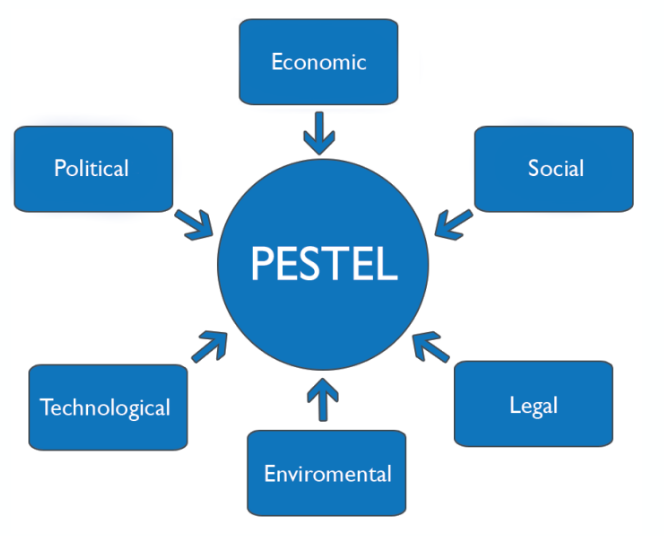
\includegraphics[width=1\linewidth]{./img/pestel}
            \captionof{figure}{5-Forces Porter}
        \end{center}
        
        \paragraph{PESTEL}
        \begin{center}
            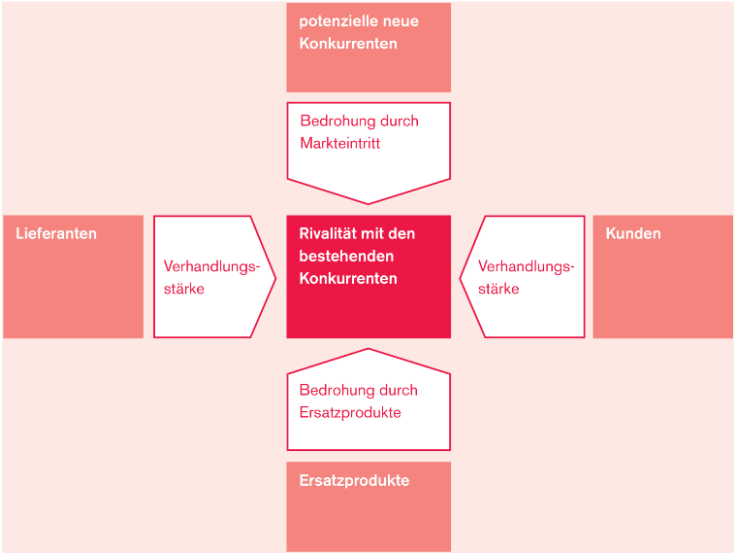
\includegraphics[width=1\linewidth]{./img/5_forces}
            \captionof{figure}{5-Forces Porter}
        \end{center}
        
        \paragraph{Generische Wettbewerbsstrategien}
        \begin{itemize}[noitemsep]
            \item Kostenführerschaft
            \item Differenzierung
            \item Nischenstrategie
        \end{itemize}
        
        \paragraph{Wachstumsstrategien}
        
        \begin{itemize}[noitemsep]
            \item Marktdurchdringung
            \item Marktentwicklung
            \item Produktentwicklung
            \item Diversifikation
        \end{itemize}
        
        \subsection{Strategische Planung}
        
        \paragraph{4 Branchen (Porter)}\mbox{}\\
        
        \begin{center}
            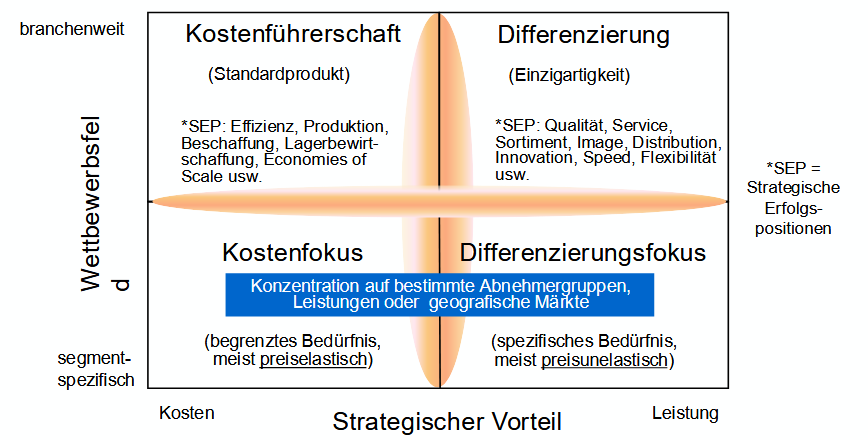
\includegraphics[width=1\linewidth]{./img/4_branchen_porter}
            \captionof{figure}{Bildbeschreibung}
        \end{center}
        
        \paragraph{4-Produkt-Markt-Strategien nach Ansoff}\mbox{}\\
        
        \begin{center}
            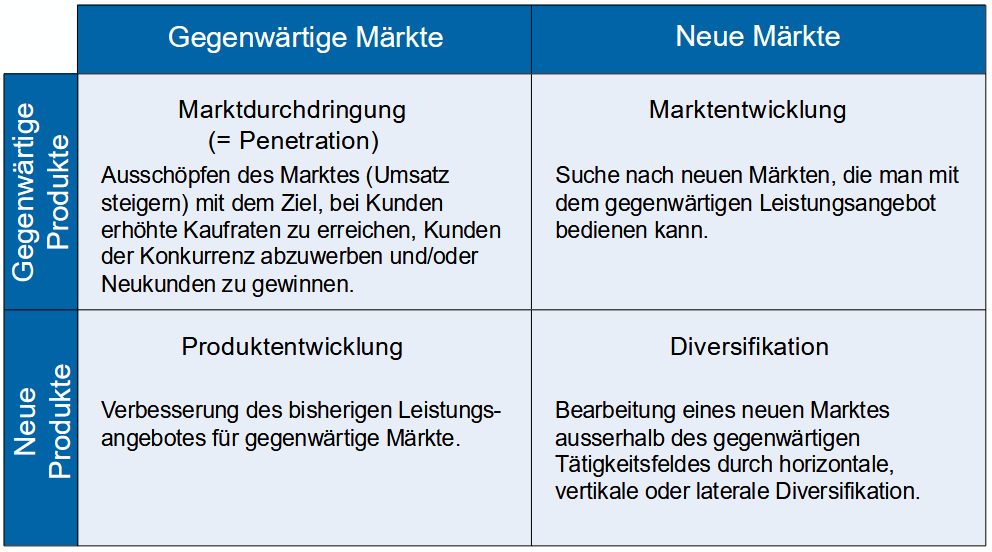
\includegraphics[width=1\linewidth]{./img/4_märkte}
            \captionof{figure}{Die vier Produkt-Markt-Strategien nach Ansoff}
        \end{center}
        
        \begin{center}
            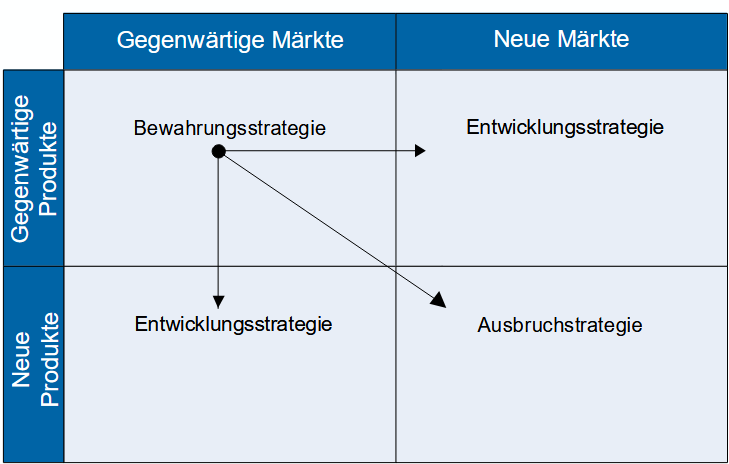
\includegraphics[width=1\linewidth]{./img/4_märkte_stossrichtungen}
            \captionof{figure}{Die drei Stossrichtungen und ihre Erfolgsaussichten}
        \end{center}
        
        \needspace{5\baselineskip}
        
        \section{Marketing}
        
        \textbf{Marketing = Analyse und Befriedigung von Kundenbedürfnissen} \\
        \textbf{Marketing: Geschäftsprozesse in SGMM}
        
        \subsection{Marktanalyse}
        \begin{itemize}[noitemsep]
            \item B2C, B2B, C2C (B=Business; C=Customer)
            \item Marktforschung: Quantitativ (Zahlen über Markt) / Qualitativ (Motive von Kunden)
            \item Erhebungsmethoden: Primär (neu Daten) / Sekundär (vorhandene Daten)
            \item Marktsegmentierung: soziodemografisch, geografisch, psychografisch, verhaltensorientiert
        \end{itemize}
        \textbf{Darstellung von Martkgrössen}
        \begin{center}
            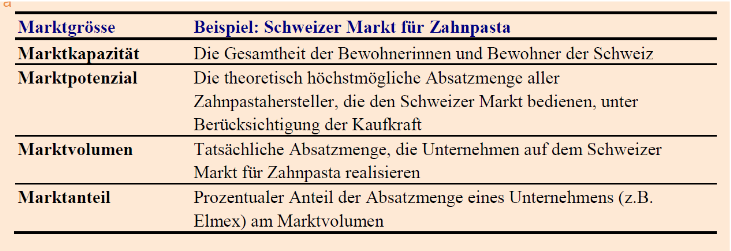
\includegraphics[width=1\linewidth]{./img/martkgrösse}
            \captionof{figure}{Marktgrössen}
        \end{center}
        $$S\text{ä}ttigungsgrad=\frac{Marktvolumen}{Marktpotenzial}*100\%$$
        
        \subsection{Marketing-Mix (4P)}
        
        \begin{center}
            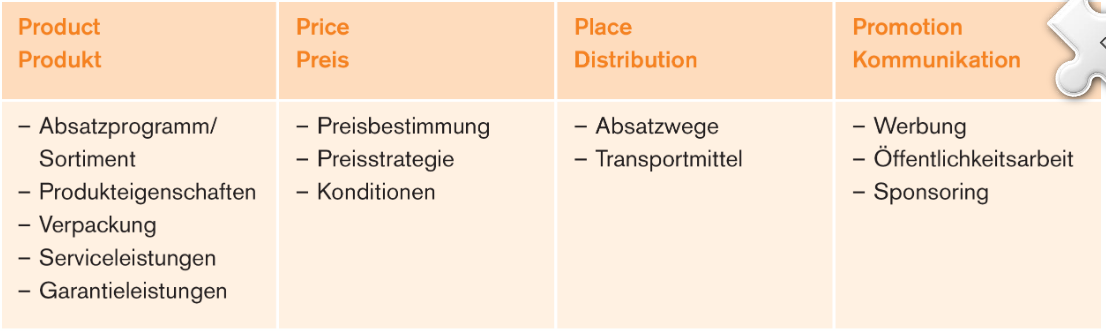
\includegraphics[width=1\linewidth]{./img/4_p}
            \captionof{figure}{4-P Marketing}
        \end{center}
        
        \subsection{Produktgestaltung}
        
        \begin{center}
            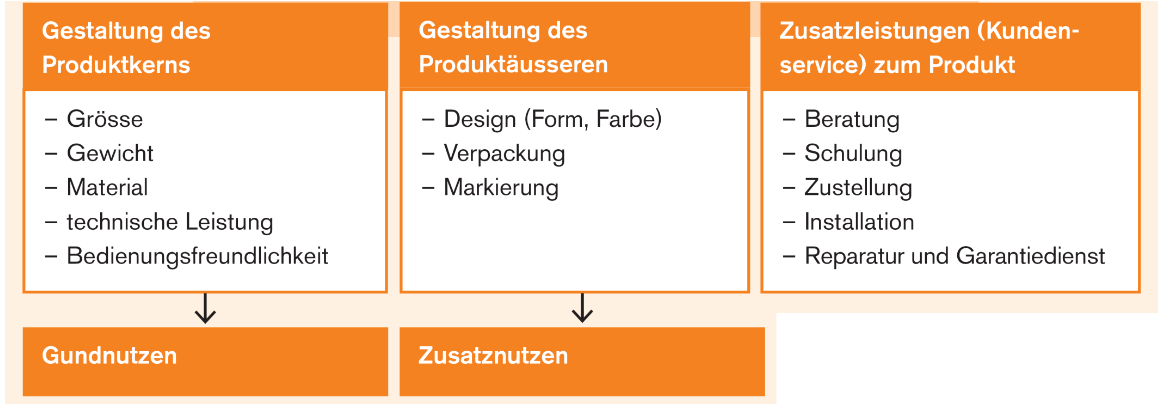
\includegraphics[width=1\linewidth]{./img/produktgestaltung}
            \captionof{figure}{produktgestaltung}
        \end{center}
        
        \subsection{Preispolitik}
        
        \begin{center}
            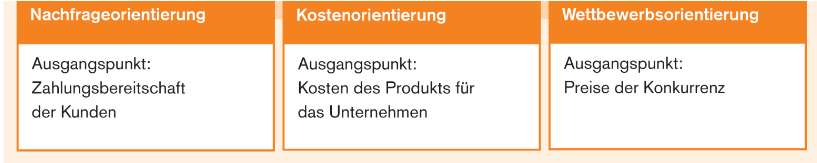
\includegraphics[width=1\linewidth]{./img/preispolitik}
            \captionof{figure}{produktgestaltung}
        \end{center}
        
        \textbf{Marke:} Signal für Qualität, Vertrauen, Wiedererkennung
        
        \textbf{CRM:} Systematische Pflege von Kundenbeziehungen zur Steigerung des Kundenwerts.
        
        \needspace{5\baselineskip}
        
        \section{Finanzen I – Bilanz \& Erfolgsrechnung}
        
        \subsection*{Bilanz}
        
        \begin{center}
        Summe der Bilanz muss auf beiden Seiten immer gleich gross sein: Aktiven = Passiven. Alle Vermögenswerte müssen immer durch Vermögensanteile gedenkt sein.\textbf{Wichtig!} Bilanz ist Stichtagbezogen. z.B. 31.12
        \end{center}
        
        \begin{multicols}{2}
            \textbf{Aktiven}
            \begin{itemize}[noitemsep]
                \item Umlaufvermögen UV
                \item Anlagevermögen AV
            \end{itemize}
            
            \textbf{Passiven}
            \begin{itemize}[noitemsep]
                \item Fremdkapital FK
                \item Eigenkapital EK
            \end{itemize}
        \end{multicols}
        Aktivkonten nehmen immer im soll zu haben ab. Passivkonten nehmen immer im haben zu und soll ab.
        
        \textbf{Geld Einzahlen (Aktivktausch)}
        
        \begin{tabular}{|c|c|c|}
            \hline
            soll & haben & Betrag \\
            \hline
            Bank & Kasse & 2000 \\
            \hline
        \end{tabular}
        
        \textbf{Kredit Aufnehmen}
        
        \begin{tabular}{|c|c|c|}
            \hline
            soll & haben & Betrag \\
            \hline
            Bank & Schulden verzinsl. langf. & 200000 \\
            \hline
        \end{tabular}
        
        \subsection{Erfolgsrechnung}
        Die ERfolgsrechnung zeigt an wie in einer gewissen Periode Geld ausgegeben oder eingenommen wurde. Summe der Aufwände und Erträge müssen immer gleich gross sein. Die Differenz ist immer der Erfolg: $\text{Erfolg} = \text{Ertrag} - \text{Aufwand}$ Erfolg kann negativ sein. Aufwandskonti nehmen im soll zu und im haben ab. Erfolgskonti nehmen im habe zu und im soll ab. \textbf{Wichtig!} Erfolgsrechnung ist immer Periodenbezogen. z.B. Jahr 2025.
        
        \begin{center}
            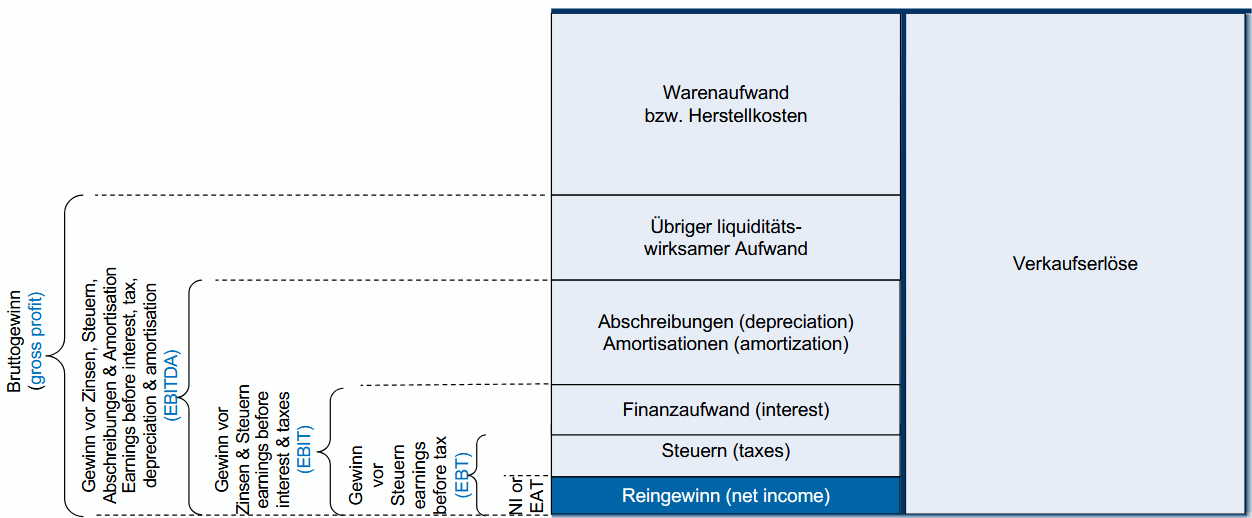
\includegraphics[width=1\linewidth]{./img/ef}
            \captionof{figure}{Erfolgsrechnung}
        \end{center}
        
        \subsection{Doppelte Buchhaltung}
        In der praxis werden Bilanz und Erfolgsrechung kombiniert daraus ergibt sich die doppelte Buchhaltung. Somit wird es möglich Vermögenswerte mit Einnahmen und Ausgaben zu veknüpfen:
        
        \textbf{Beispiel: Rechnung bezahlen}
        
        \begin{tabular}{|c|c|c|c|}
            \hline
            Datum & soll & haben & Betrag \\
            \hline
            01.12 & Getränkeaufwand & Kreditor & 1500 \\
            \hline
            13.12 & Kreditor & Bank & 1500 \\
            \hline
        \end{tabular}\\
        \textbf{Kommentar}: Aufwand wird beim erhalten der Rechnung verbucht. Der reguläre Rechnungslauf findert aber erst 2 Wochen später statt. 
        
        \section{Finanzen II – Cashflow \& Kennzahlen}
        
        \subsection{Cashflow}
        Ziel des Geldflussrechnung ist es, zu zeigen wie sich die flüssigen Mittel inerhalb eine bestimmten Periode verändert haben. Nebst Bilanz und EF wichtigstes Tool zur Ermittlung der Unternehmensfinanzen. Firmen könne Konkurs gehen obwohl sie viel Vermögenswerte haben, weil kein Geld um Rechnungen zu bezahlen. Mit Immobilien und Aktien kann man keine Rechnungen bezahlen.\\
        \textbf{Beispiel: Geldflussrechnung (direkte Methode)}
        \begin{center}
            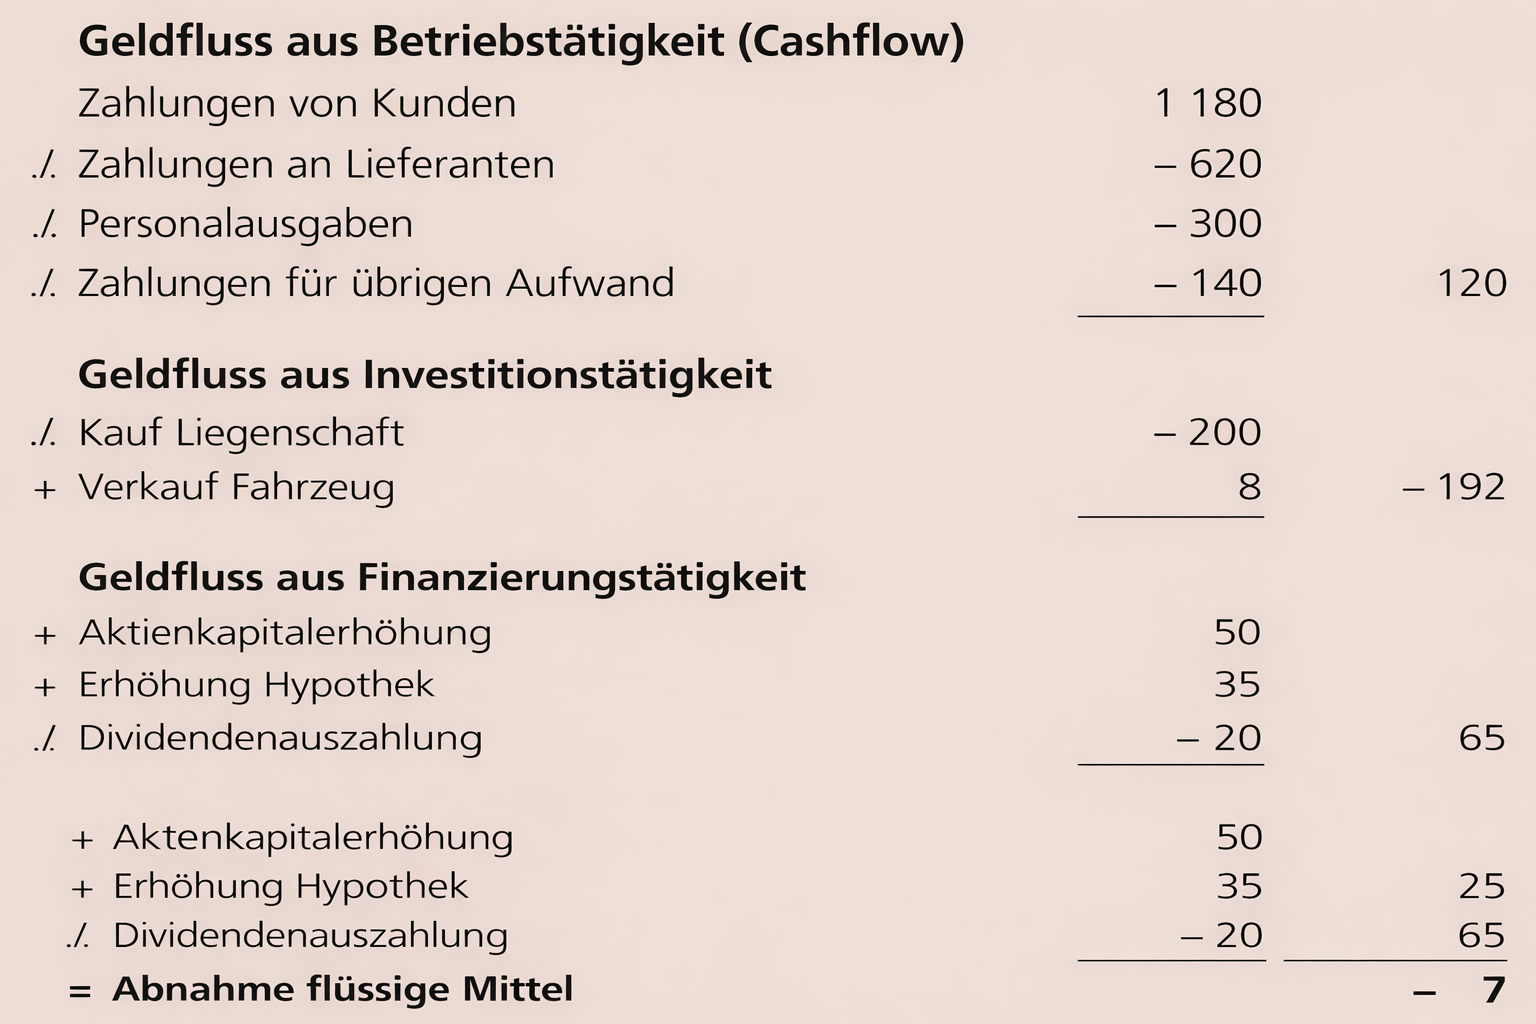
\includegraphics[width=0.8\linewidth]{./img/cashflow}
            \captionof{figure}{Cashflow}
        \end{center}
        \textbf{Beispiel: Schemata}
        \begin{center}
            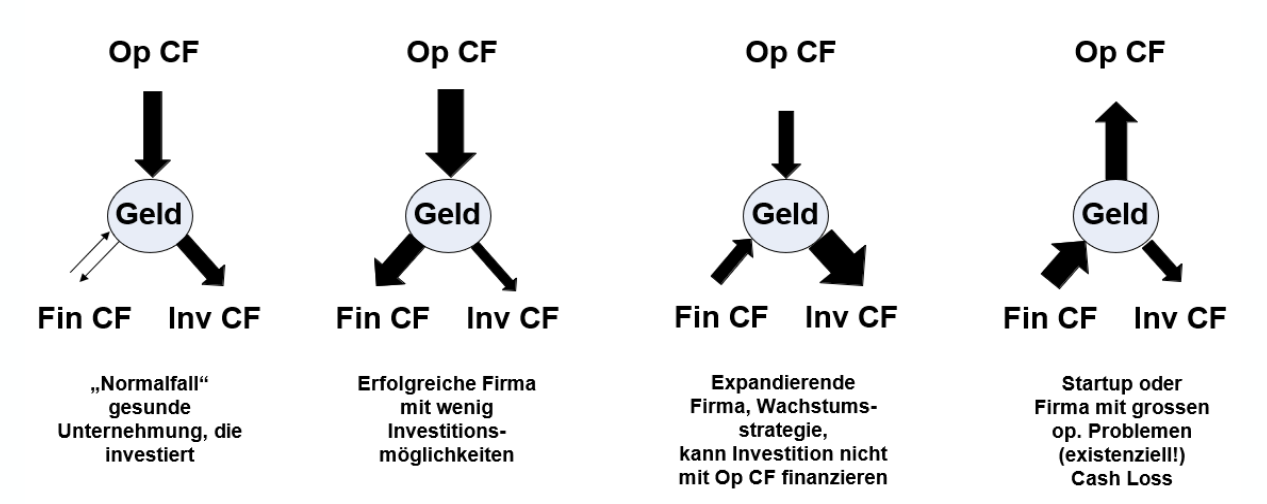
\includegraphics[width=1\linewidth]{./img/cashflow_schemata}
            \captionof{figure}{Cashflow Schemata}
        \end{center}
        \begin{itemize}[noitemsep]
            \item Cashflow aus Betriebstätigkeit
            \item Cashflow aus Investitionstätigkeit
            \item Cashflow aus Finanzierungstätigkeit
        \end{itemize}
        \textbf{Cashfoow (indirekte Methode)}
        Bei der indirekten Methode werden die Geldflüsse aus der Bilanz gelesen: z.B. Vergleich Flüssigmittel vor einem Jahr und jetzt. Wenn alles saube gebucht wurde, CF-direkt = CF-indirekt.
        
        \subsection{Investitionsdreieck}
        \begin{center}
            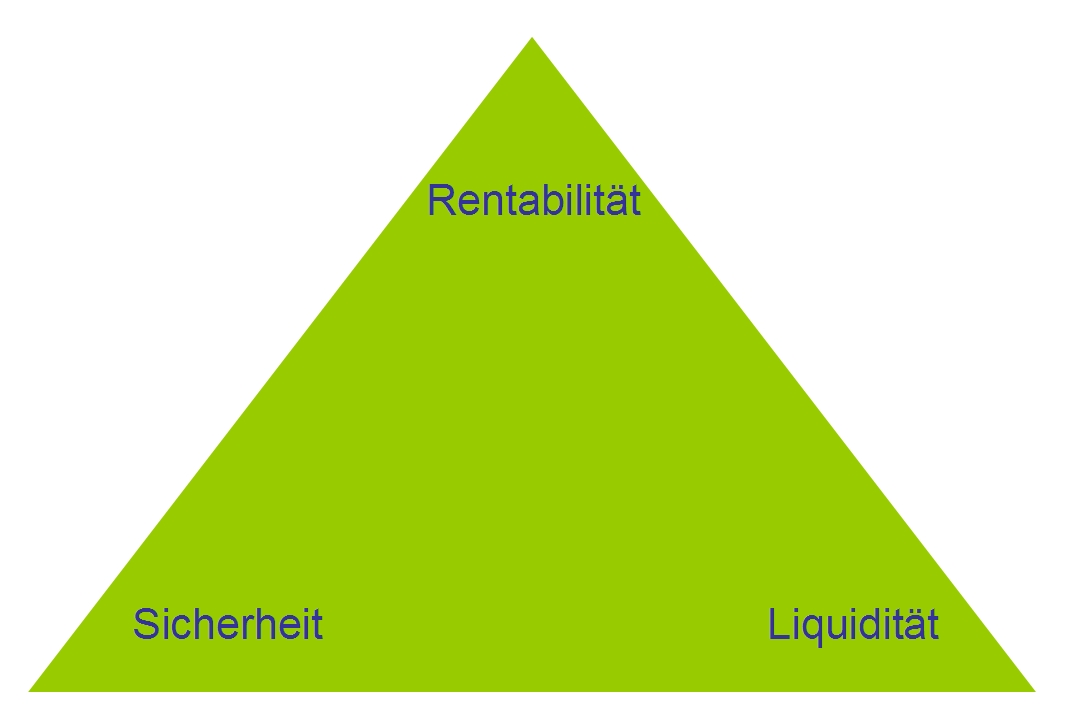
\includegraphics[width=0.6\linewidth]{./img/investitionsdreieck}
            \captionof{figure}{investitionsdreieck}
        \end{center}
        
        \subsection{Kennzahlen-Liquidität}
        
        \textbf{Liquiditätsgrad I}\\
        Richtwert $> 20\%$
        $$\frac{\text{Flüssige Mittel}}{\text{kurzfr. Fremdkapital}}$$
        
        \textbf{Liquiditätsgrad II}\\
        Richtwert $100\%$
        $$\frac{\text{Flüssige Mittel + Forderungen}}{\text{kurzfr. Fremdkapital}}$$
        
        \textbf{Eigenkapitalquote}\\
        Richtwert $150\%-200\%$
        $$\frac{\text{Eigenkapital}}{\text{Gesamtkapital}}$$
        
        \subsection{Kennzahlen-Sicherheit}
        
        \textbf{Eigenkapitalquote}\\
        Richtwert $> 30\%$
        $$\frac{\text{Eigenkapital}}{\text{Gesamtkapital}} \cdot 100\%$$
        
        \textbf{Fremdkapitalquote}\\
        Richtwert $< 70\%$
        $$\frac{\text{Fremdkapital}}{\text{Gesamtkapital}} \cdot 100\%$$
        
        \textbf{Verschuldungsgrad}\\
        Richtwert $< 230\%$
        $$\frac{\text{Fremdkapital}}{\text{Eigenkapital}} \cdot 100\%$$
        
        \textbf{Anlagedeckungsgrad I}\\
        Richtwert $90-120\%$
        $$\frac{\text{Eigenkapital}}{\text{Anlagevermögen}} \cdot 100\%$$
        
        \textbf{Anlagedeckungsgrad II}\\
        Richtwert $120-160\%$
        $$\frac{\text{Eigenkapital} + \text{langfristiges Fremdkapital}}
        {\text{Anlagevermögen}} \cdot 100\%$$
        
        \section{Betriebsbuchhaltung (Voll- und Teilkostenrechnung)}
        
        \subsection{Vollkostenrechnung}
        
        \begin{center}
            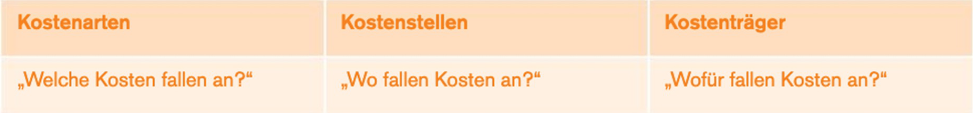
\includegraphics[width=1\linewidth]{./img/vollkostenrechnung_begriffe}
            \captionof{figure}{Vollkostenrechnung}
        \end{center}
        
        \textbf{Betriebsabrechnungsbogen (BAB):}
        \begin{center}
            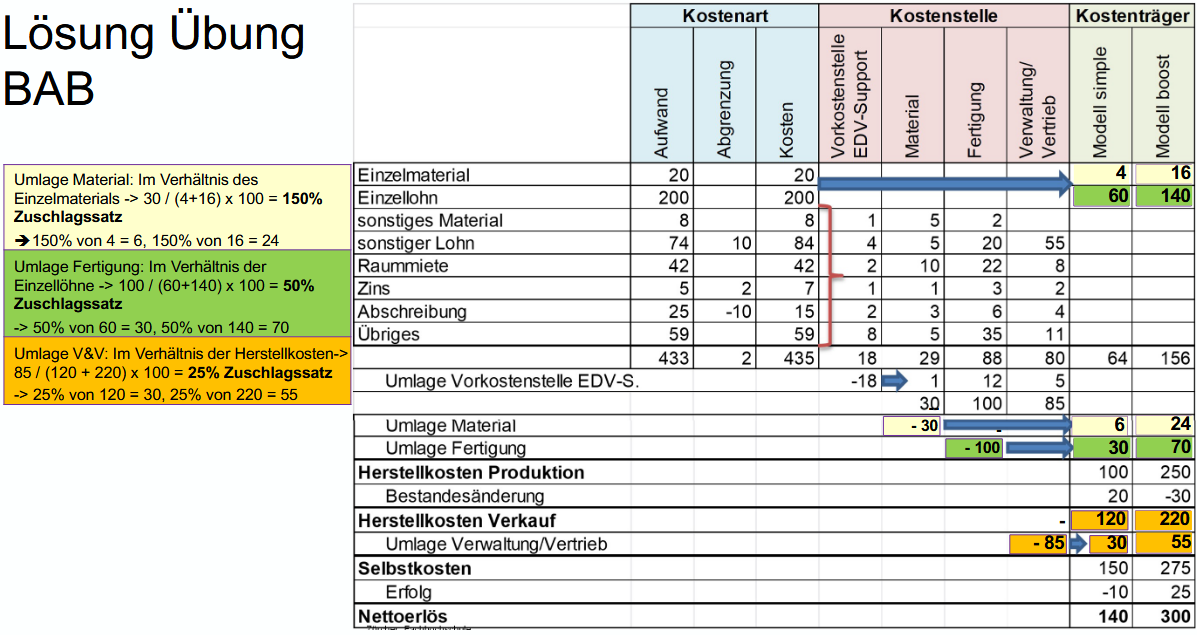
\includegraphics[width=1\linewidth]{./img/bab}
            \captionof{figure}{BAB}
        \end{center}
        
        \textbf{Zuschlagssatz}
        $$\frac{\text{Endstellenkosten (ESK) der Hauptkostenstelle}}
        {\text{Bezugsgröße der Hauptkostenstelle}}
        \cdot 100\%$$
        \textbf{Materialgemeinkostenzuschlagssatz}
        $$\frac{\text{Materialgemeinkosten}}
        {\text{Materialeinzelkosten}}
        \cdot 100\%$$
        \textbf{Fertigungsgemeinkostenzuschlagssatz}
        $$\frac{\text{Fertigungsgemeinkosten}}
        {\text{Fertigungseinzelkosten}}
        \cdot 100\%$$
        \textbf{Verwaltungskostenzuschlagssatz}
        $$\frac{\text{Verwaltungskosten}}
        {\text{Herstellkosten}}
        \cdot 100\%$$
        \textbf{Vertriebsgemeinkostenzuschlagssatz}
        $$\frac{\text{Vertriebsgemeinkosten}}
        {\text{Herstellkosten}}
        \cdot 100\%$$
        
        \subsection{Teilkostenrechnung}
        \begin{center}
            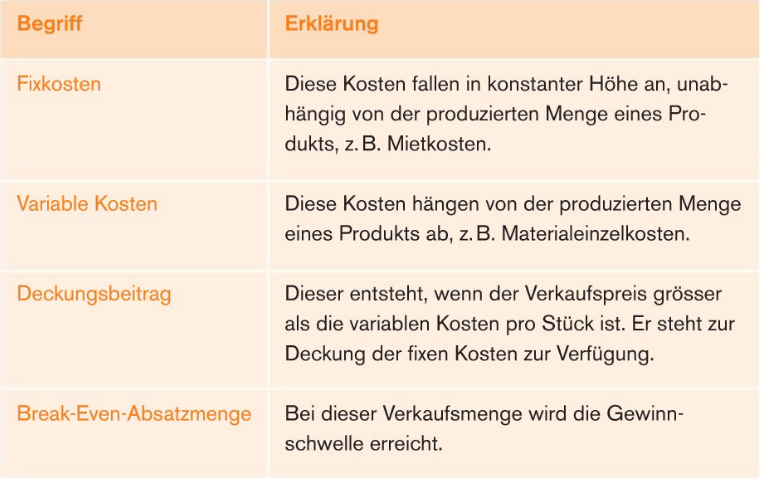
\includegraphics[width=1\linewidth]{./img/teilkostenrechnung}
            \captionof{figure}{teilkostenrechnung}
        \end{center}
        \textbf{Deckungsbeitrag}
        
        $$\text{Nettoerlös(Verkaufspreis)} - \text{variable Kosten}$$
        
        \textbf{Break-even-Menge}
        $$x_{BE} = \frac{\text{Fixkosten}}{Deckungsbeitrag/Stk.}$$
        
        \section{Kalkulation}
        
        \subsection{Industriebetrieb}
        Zusätzlich zum BAB kommen jetzt noch Steuern, Rabatt, etc auf den Nettoerlös drauf. Die zuschalgsätze und der BAB dienen hier wieder als Basis.
        \begin{center}
            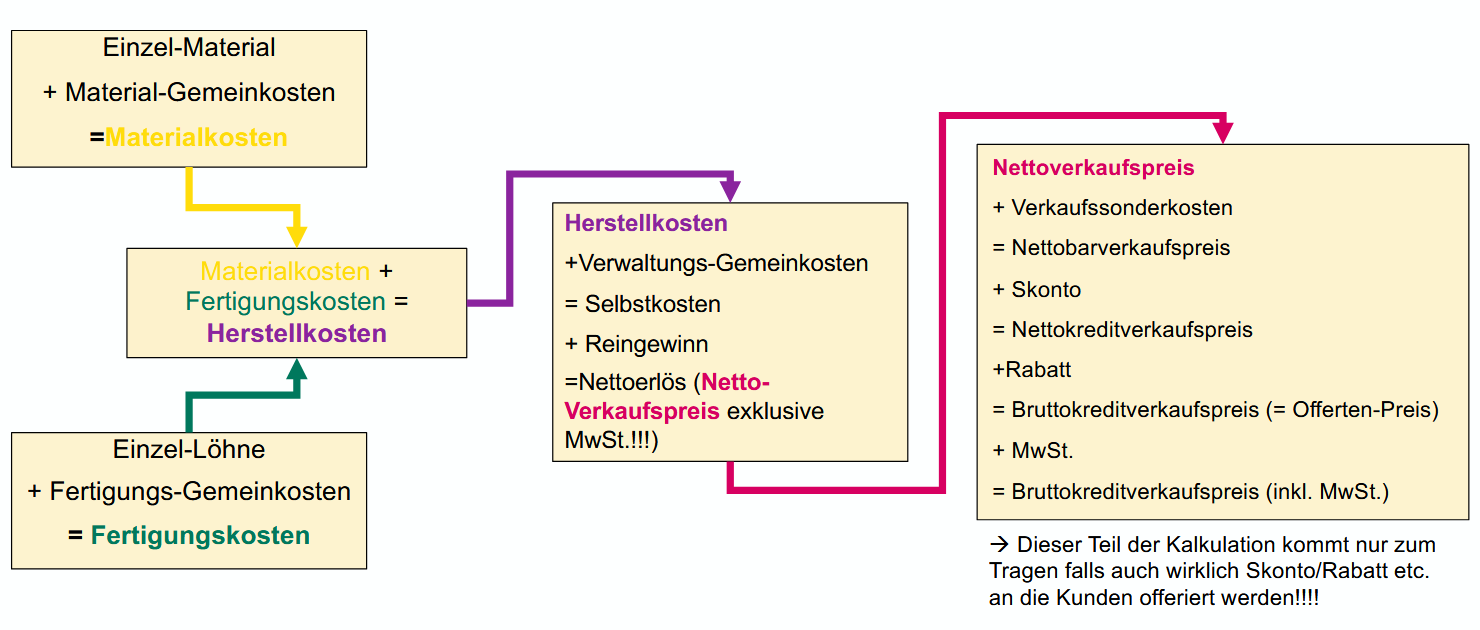
\includegraphics[width=1\linewidth]{./img/kalkulation}
            \captionof{figure}{kalkulation}
        \end{center}
        
        \subsection{Handelsbetrieb – Dreistufige Kalkulation}
        
        \begin{center}
            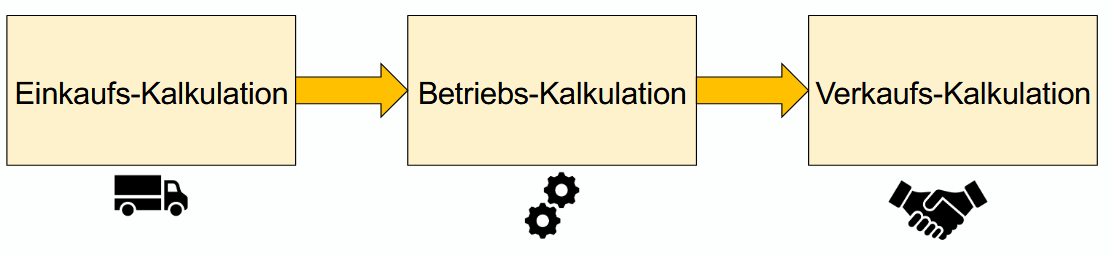
\includegraphics[width=1\linewidth]{./img/kalkulation_handel}
            \captionof{figure}{kalkulation handel}
        \end{center}
        
        \begin{center}
            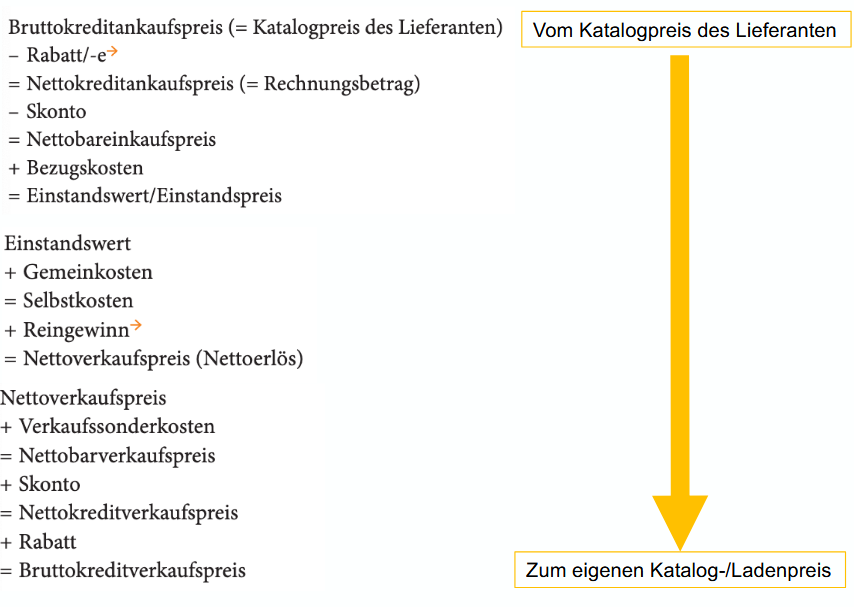
\includegraphics[width=1\linewidth]{./img/kalkulation_handel_beispiel}
            \captionof{figure}{kalkulation handel}
        \end{center}
        
        \section{Materialwirtschaft}
        Geschäftsprozess im SGMM
        Materialwirtschaft ist für die Verwaltung, Planung und Steuerung der Materialbewegungen
        innerhalb eines Unternehmens und zwischen dem Unternehmen und seiner Umwelt zuständig
        und erfüllt zwei Aufgaben:
        
        \begin{center}
            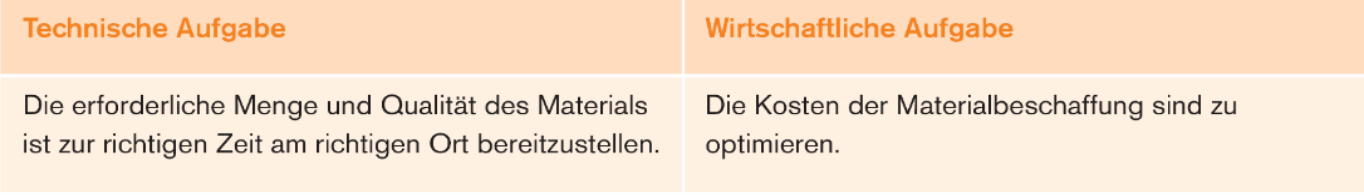
\includegraphics[width=1\linewidth]{./img/materialwirtschaft_1}
            \captionof{figure}{Aufgaben Materialwirtschaft}
        \end{center}
        
        \subsection{Bestandteile}
        \begin{center}
            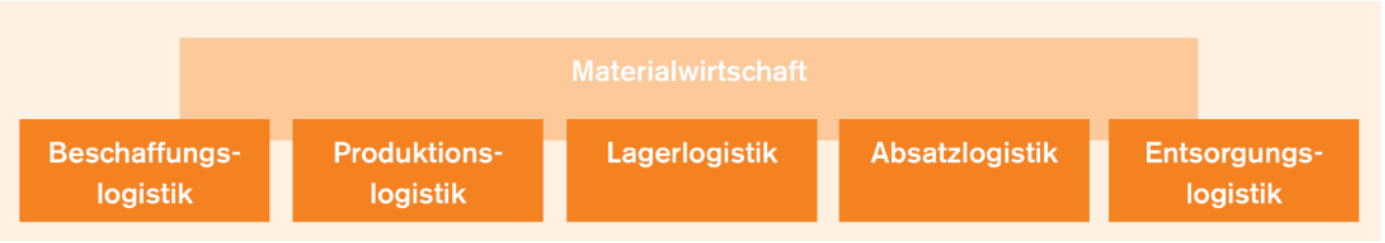
\includegraphics[width=1\linewidth]{./img/materialwirtschaft_bestandteile}
            \captionof{figure}{Bestandteile Materialwirtschaft}
        \end{center}
        
        \subsection{Beschaffungsprozesse}
        \begin{center}
            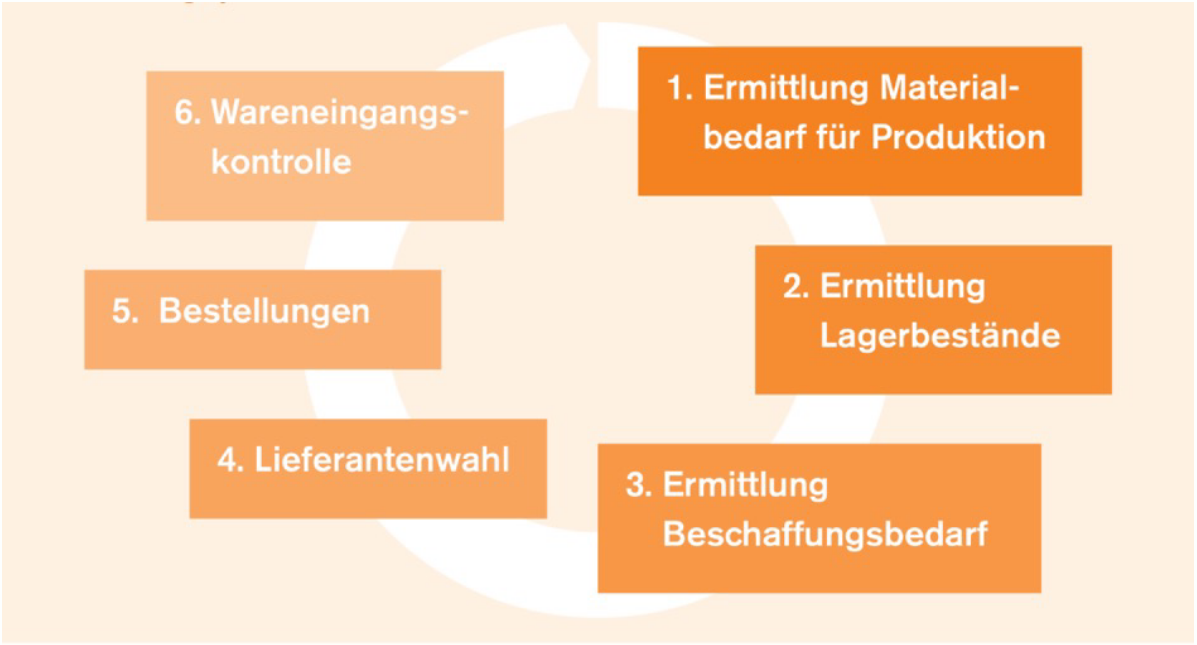
\includegraphics[width=1\linewidth]{./img/beschaffungsprozesse}
            \captionof{figure}{Beschaugnsprozesse}
        \end{center}
        
        \subsection{Beschaffungsobjekte}
        \begin{center}
            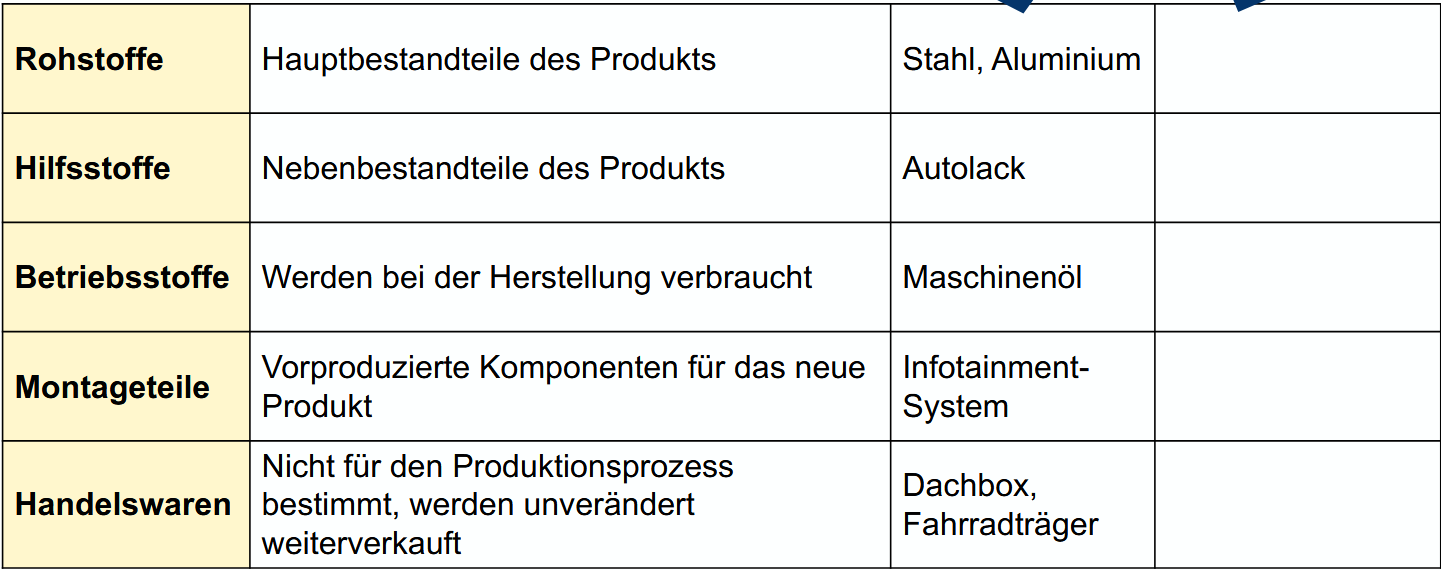
\includegraphics[width=1\linewidth]{./img/beschaffungsobjekte}
            \captionof{figure}{Beschaffungsobjekte}
        \end{center}
        
        \subsection{Beschaffungskonzepte}
        \begin{itemize}[noitemsep]
            \item Voratsbeschaffung (Lager)
            \item Fallweisebeschaffung (on Demand - Lager Liefertant)
            \item JIT (Just int Time - kein Lager)
            \item JIS (Just in Sequnence - Direkt an Produktion)
        \end{itemize}
        
        \subsection{magisches Dreieck Materialwirtschaft}
        \begin{center}
            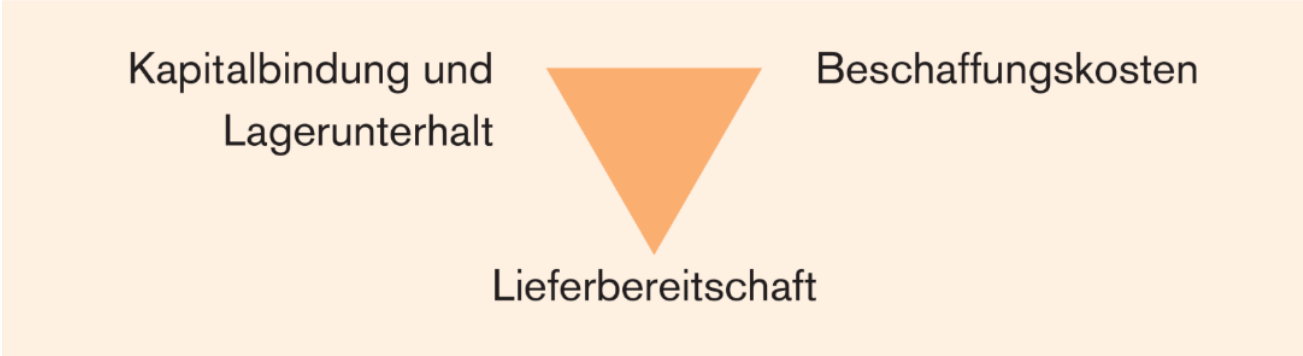
\includegraphics[width=1\linewidth]{./img/dreieck_material}
            \captionof{figure}{magisches Dreieck}
        \end{center}
        
        \subsection{ABC-Analysse (Pareto-Prinzip)}
        \begin{center}
            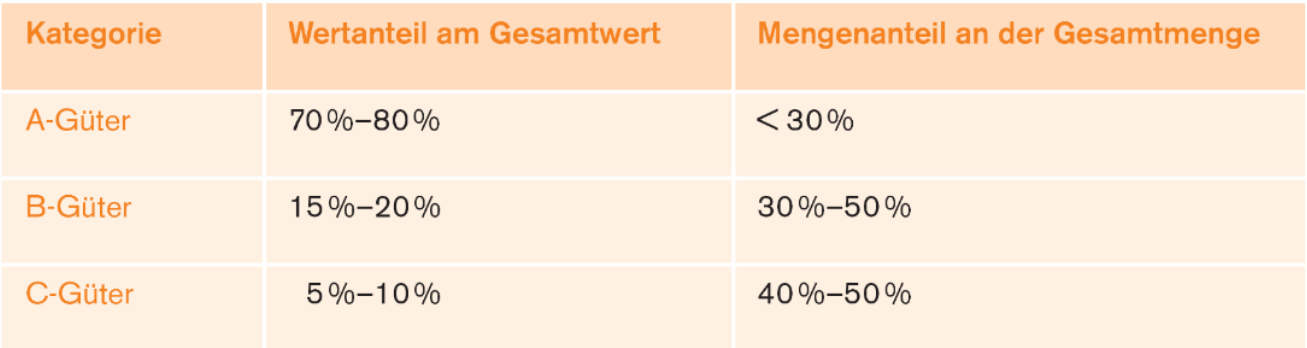
\includegraphics[width=1\linewidth]{./img/abc}
            \captionof{figure}{abc}
        \end{center}
        
        \subsection{XYZ-Analysse (Vorhersagebarkeit)}
        \begin{center}
            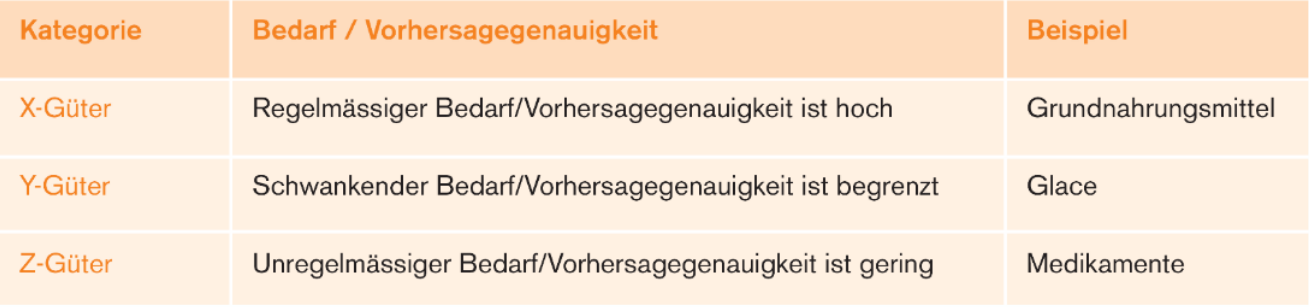
\includegraphics[width=1\linewidth]{./img/xyz}
            \captionof{figure}{xyz}
        \end{center}
        
        \subsection{Lagerlogistik / Lagerfunktion}
        \begin{itemize}[noitemsep]
            \item Zeitüberbrückung
            \item Sicherung
            \item Speckulation
            \item Veredlung und Umformung
            \item Assortierung (Sammellieferung und Präsentation)
        \end{itemize}
        
        \subsection{Durchschnittlicher Lagerbestand}
        \textbf{Vertriebsgemeinkostenzuschlagssatz}
        $$\frac{\text{Anfangsbestand} + \text{Endbestand}}{2}$$
        \textbf{Lagerumschlagshäufigkeit}
        $$\frac{\text{Jahresverbrauch}}
        {\text{durchschnittlicher Lagerbestand}}$$
        \textbf{Durchschnittliche Lagerdauer}
        $$\frac{360}{\text{Lagerumschlagshäufigkeit}}$$
        
        \section{Personalmanagement}
        Unterstützungsprozesse - SGMM
        \subsection{Hauptaufgaben}
        \begin{center}
            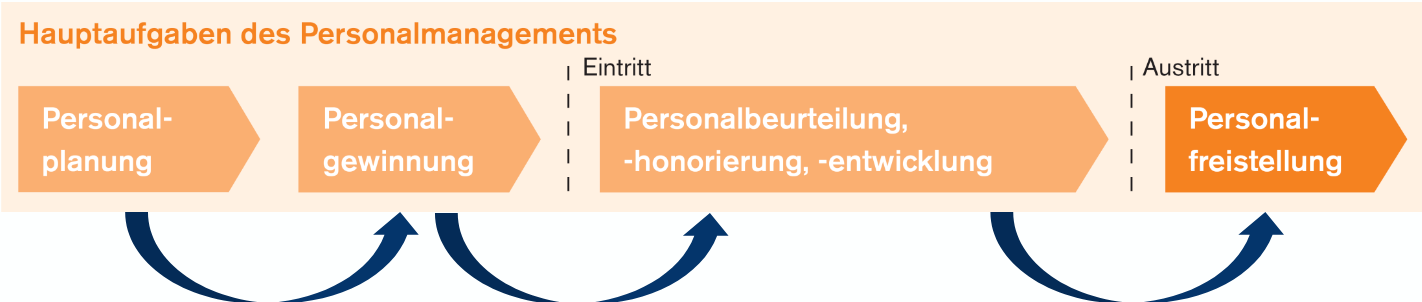
\includegraphics[width=1\linewidth]{./img/aufgaben_personalmanagement}
            \captionof{figure}{Aufgaben Personalmanagement}
        \end{center}
        \subsection{Personalplanung}
        \begin{center}
            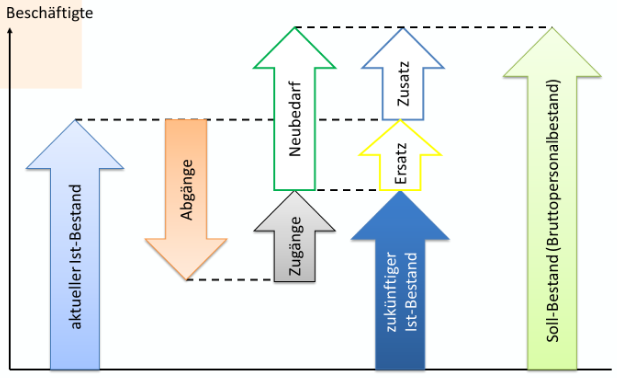
\includegraphics[width=1\linewidth]{./img/personalplanung}
            \captionof{figure}{Personalplanung}
        \end{center}
        
        \textbf{Fragestellung Personalplanung}
        \begin{itemize}[noitemsep]
            \item inhaltliche, fachliche Ziele
            \item Aufgaben
            \item Qualifikationen
            \item Mittel
            \item Stelle
            \item persönliche Merkmale (selbst und Team)
        \end{itemize}
        
        \subsection{Personalgewinnung}
        \begin{center}
            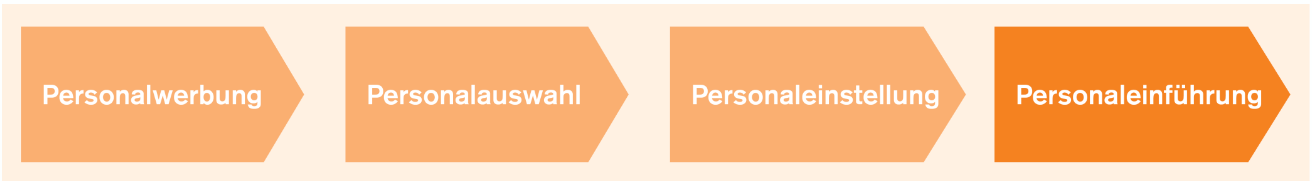
\includegraphics[width=1\linewidth]{./img/personalgewinnung}
            \captionof{figure}{personalgewinnung}
        \end{center}
        intere Personalgewinnung \textbf{vs} externe Personalgewinnung
        
        \subsection{Kirterien Personalauswahl}
        \begin{center}
            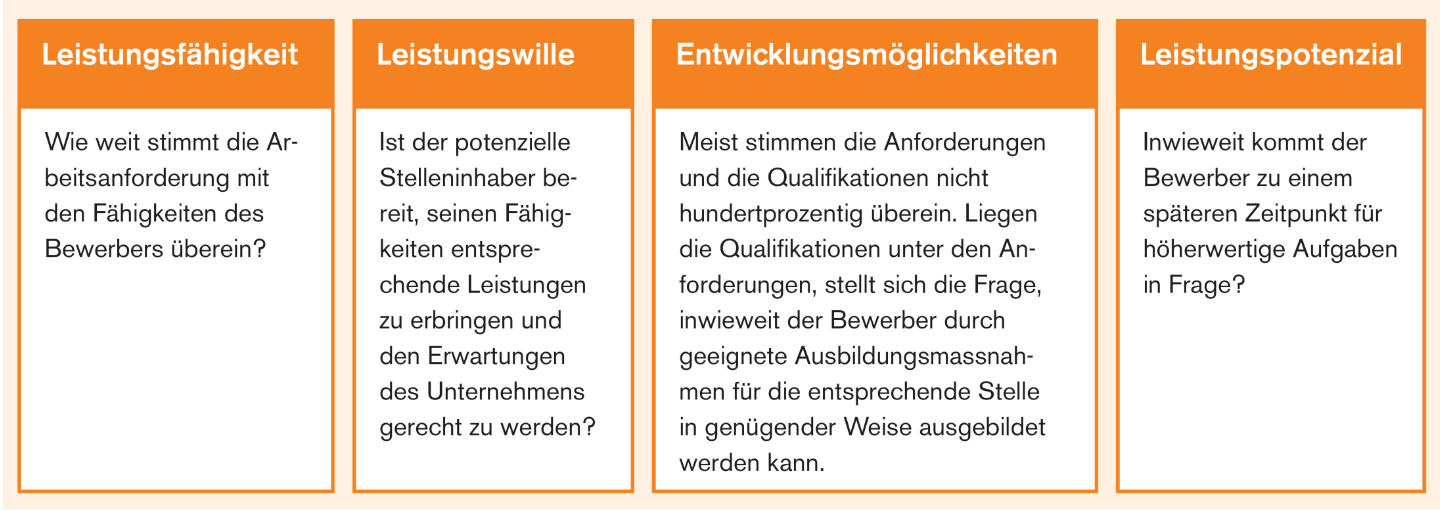
\includegraphics[width=1\linewidth]{./img/kriterien_personal}
            \captionof{figure}{Kriterien bei der Personalauswahl}
        \end{center}
        
        \subsection{Personalentwicklung}
        
        \textbf{Kompetenzentorietierung}
        \begin{center}
            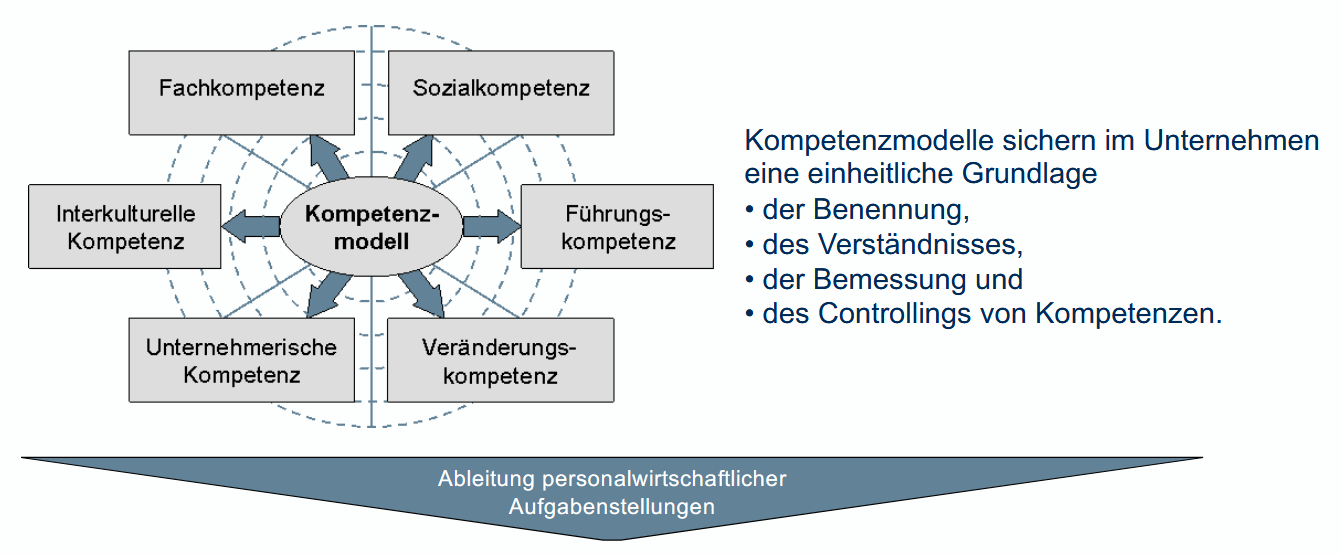
\includegraphics[width=1\linewidth]{./img/personalentwicklung_kompetenz}
            \captionof{figure}{Kompetenz}
        \end{center}
        
        \textbf{360°}
        \begin{center}
            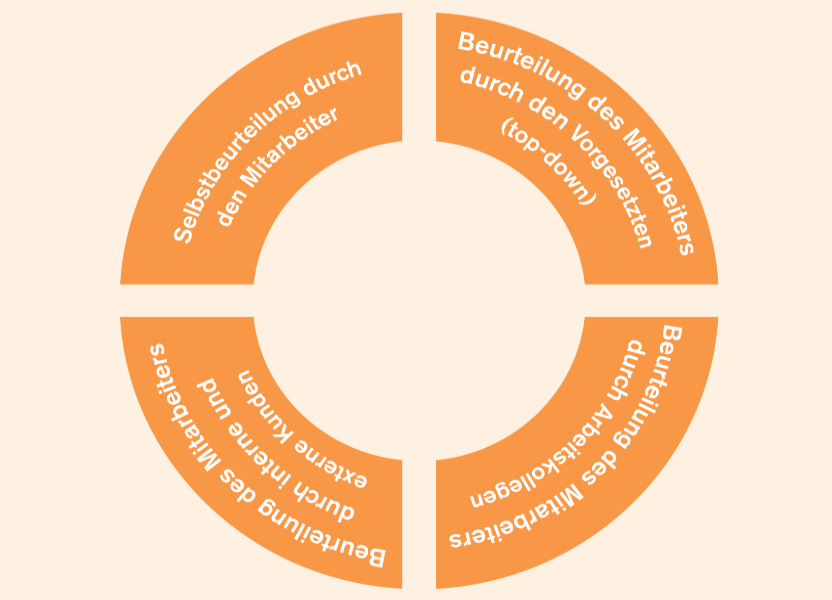
\includegraphics[width=1\linewidth]{./img/personalentwicklung_360}
            \captionof{figure}{360}
        \end{center}
        
        \subsection{Personalhonorierung}
        \begin{center}
            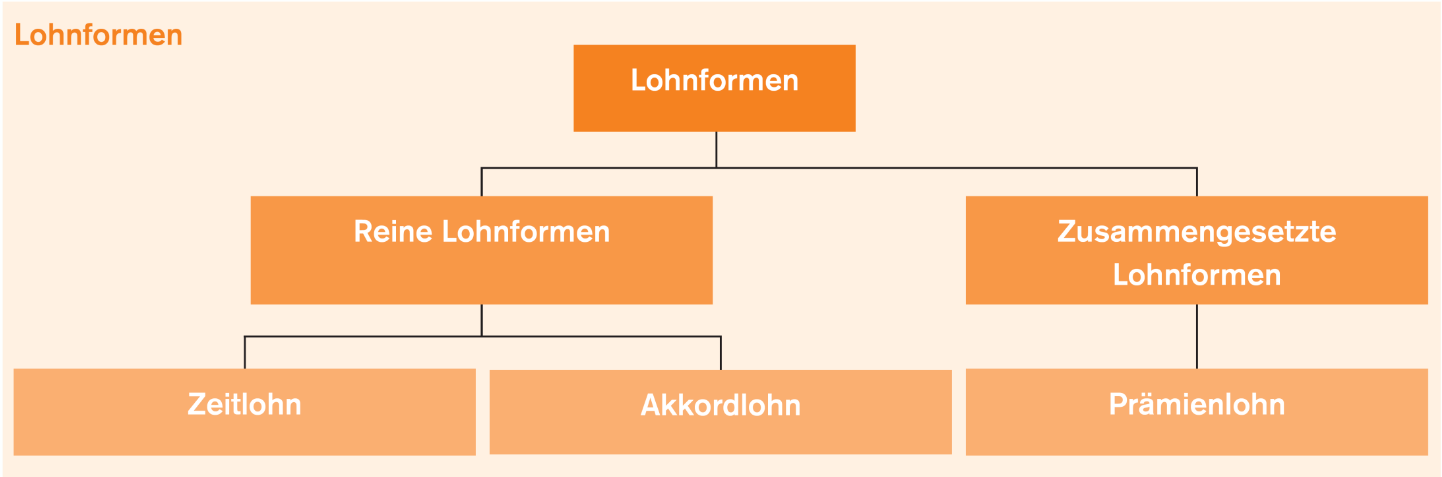
\includegraphics[width=1\linewidth]{./img/lohn}
            \captionof{figure}{lohn}
        \end{center}
        
        \section{Investitionsrechnung}
        Eine Investition ist eine Zahlungsreihe mit einer anfänglichen Auszahlung und späteren Einzahlungen.
        Ziel: Optimale Verwendung des knappen Kapitals.
        
        \begin{itemize}
            \item Aufwand/Ertrag $\neq$ Auszahlung/Einzahlung
            \item Investitionsrechnung arbeitet mit \textbf{Zahlungsströmen}
        \end{itemize}
        
        \textbf{Investitionsgründe}
        \begin{itemize}
            \item Normativ
            \item Strategisch
        \end{itemize}
        
        \begin{center}
            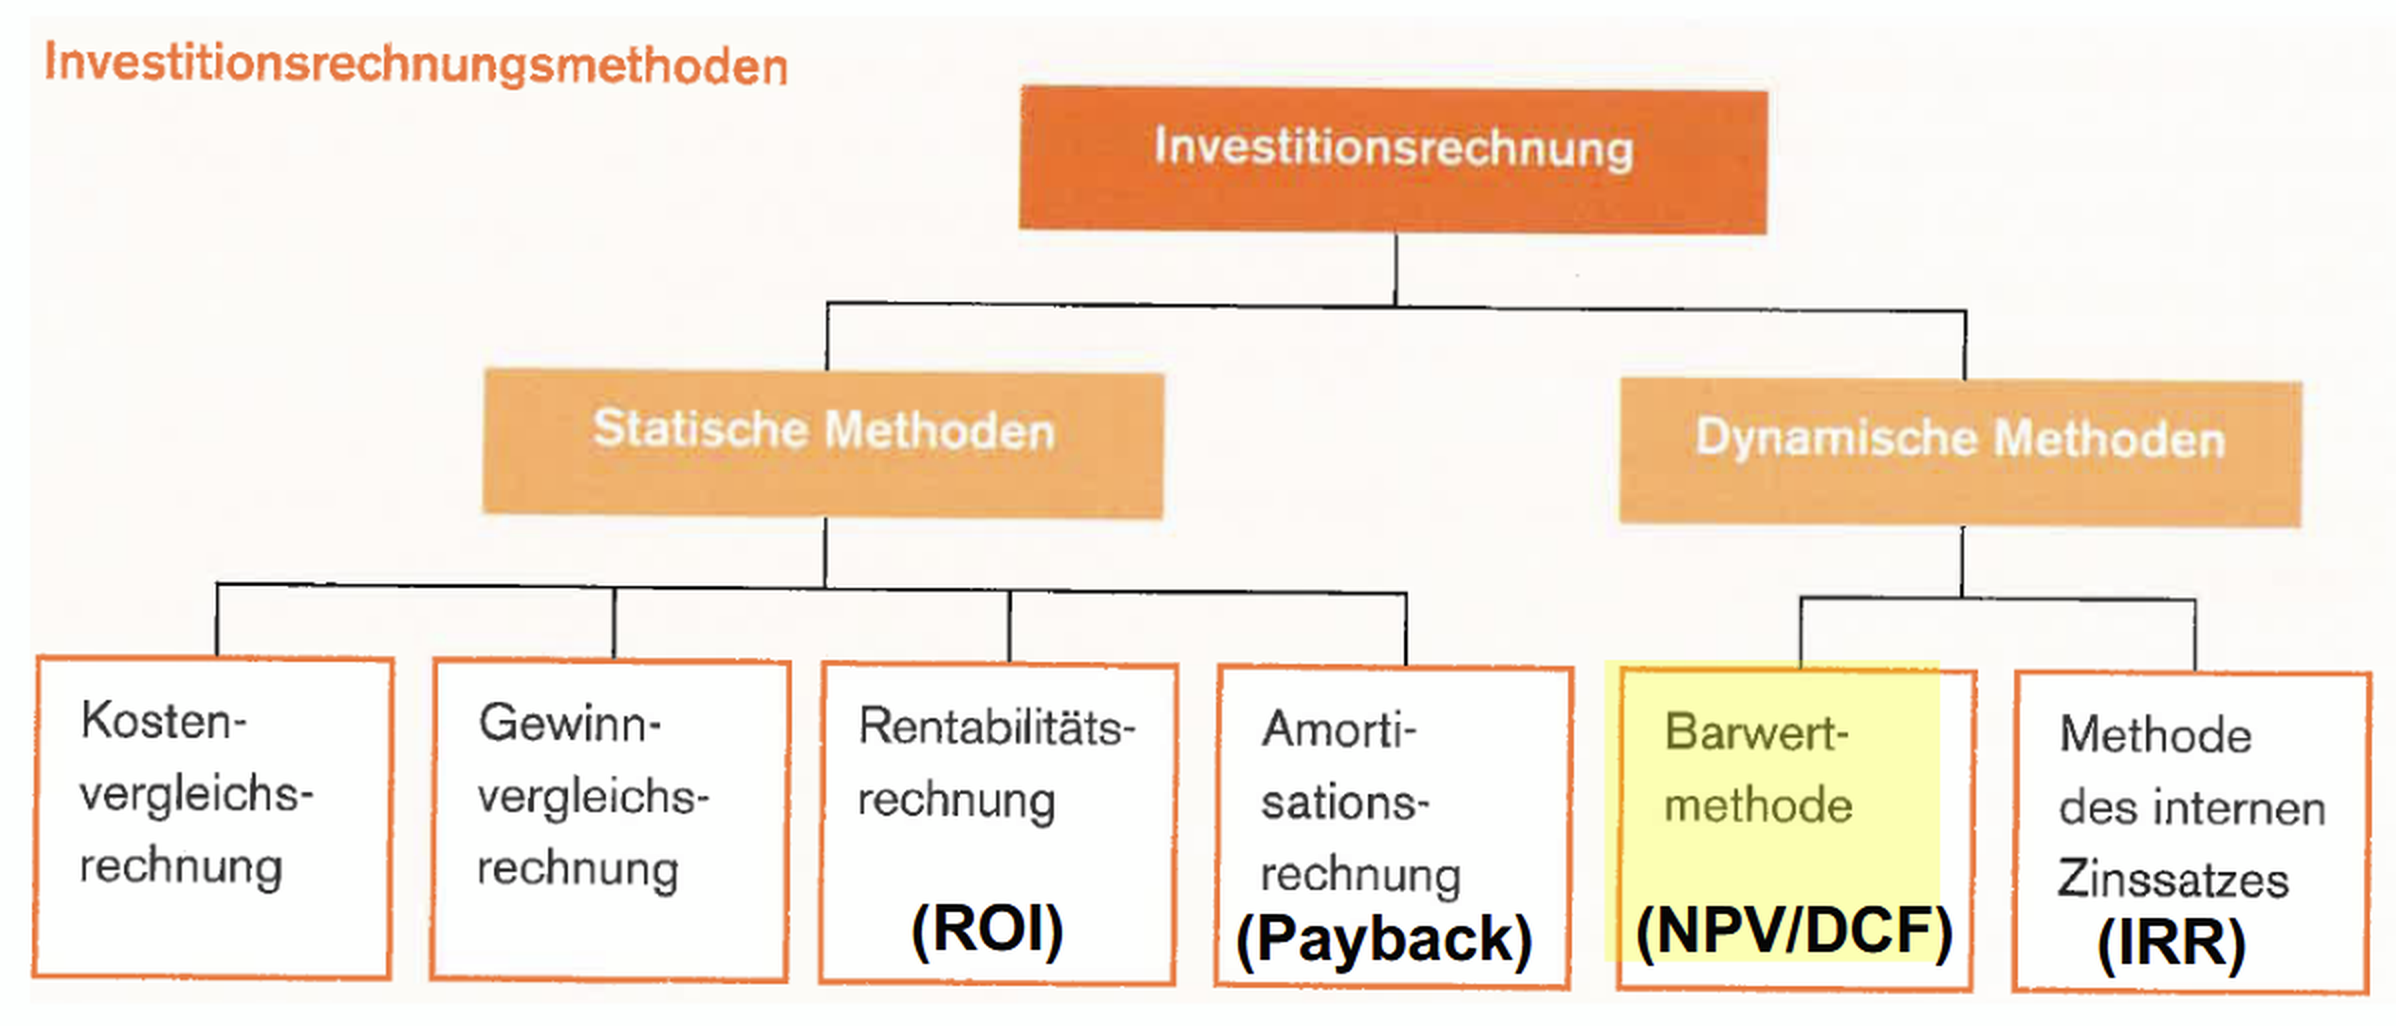
\includegraphics[width=1\linewidth]{./img/investitionsrechnung}
            \captionof{figure}{investitionsrechnung}
        \end{center}
        
        \subsection{Statische Verfahren}
        Vergleich ohne Zins.
        \begin{center}
            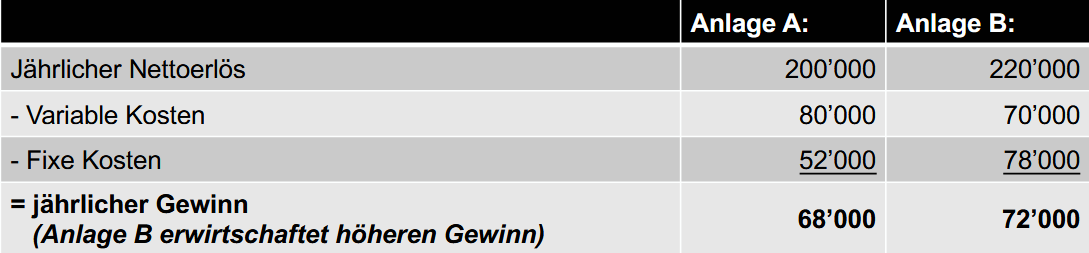
\includegraphics[width=1\linewidth]{./img/statisch_1}
            \captionof{figure}{statisch}
        \end{center}
        \subsubsection{Kostenvergleich}
        $$K = K_{\text{variabel}} + K_{\text{fix}}$$
        Entscheid: minimale Gesamtkosten.
        
        \subsubsection{Gewinnvergleich}
        $$Gewinn = Netterl\text{ö}s - Kosten_{Gesamt}$$
        Entscheid: maximaler Gewinn.
        
        \subsubsection{Rentabilität (ROI)}
        $$\text{ROI} = \frac{G + Z_{\text{kalk}}}{K_{\text{eingesetzt}}} \cdot 100$$
        Entscheid: höchste Rentabilität.
        
        \subsubsection{Amortisationsrechnung (Payback)}
        $$t_{avg} = \frac{\text{Investition}}{\text{jährlicher Cashflow}}$$
        Entscheid: kürzeste Rückzahlungsdauer.
        
        \subsection{Dynamische Verfahren}
        
        \subsubsection{Aufzinsung}
        \begin{center}
            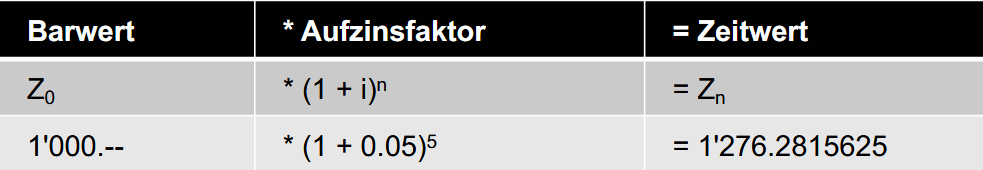
\includegraphics[width=1\linewidth]{./img/aufzinsung}
            \captionof{figure}{aufzinsung}
        \end{center}
        
        \subsubsection{Abzinsung}
        \begin{center}
            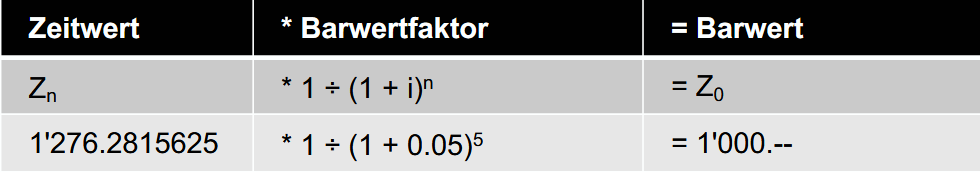
\includegraphics[width=1\linewidth]{./img/abzinsung}
            \captionof{figure}{aufzinsung}
        \end{center}
        \subsubsection{Kapitalwertmethode (NPV)}
        \begin{center}
            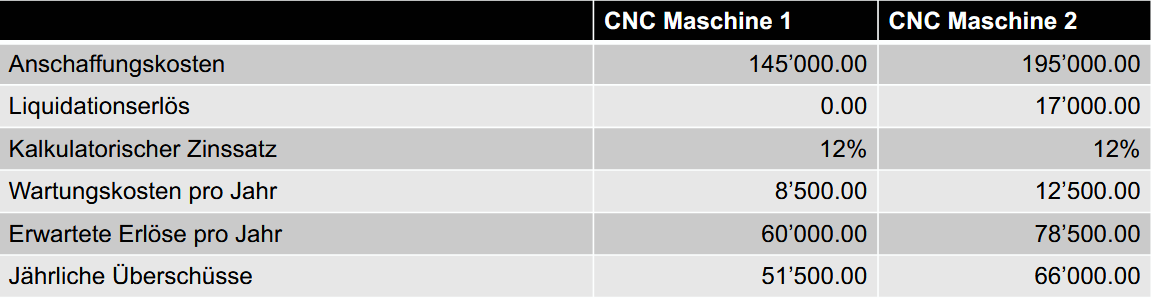
\includegraphics[width=1\linewidth]{./img/npv_1}
            \captionof{figure}{npv}
        \end{center}
        \begin{center}
            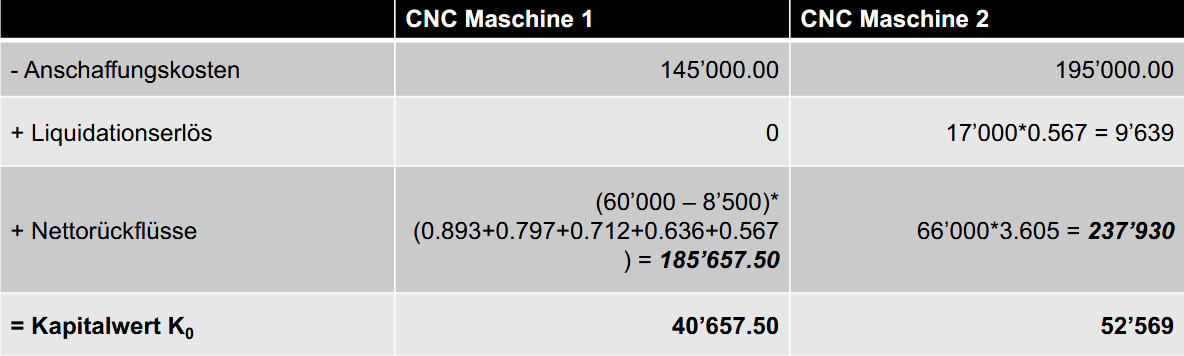
\includegraphics[width=1\linewidth]{./img/npv_2}
            \captionof{figure}{npv}
        \end{center}
        Die Zinssätze für das Abzines entnehmen wir aus der Abzinsungstabelle. \\
        \textbf{Entscheid:}
        \begin{itemize}
            \item NPV $>0$: Investition vorteilhaft
            \item Höchster NPV bevorzugt
        \end{itemize}
        
        \section{Realisation}
        
        \subsection{Wertschöpfungsmanagement}
        \begin{center}
            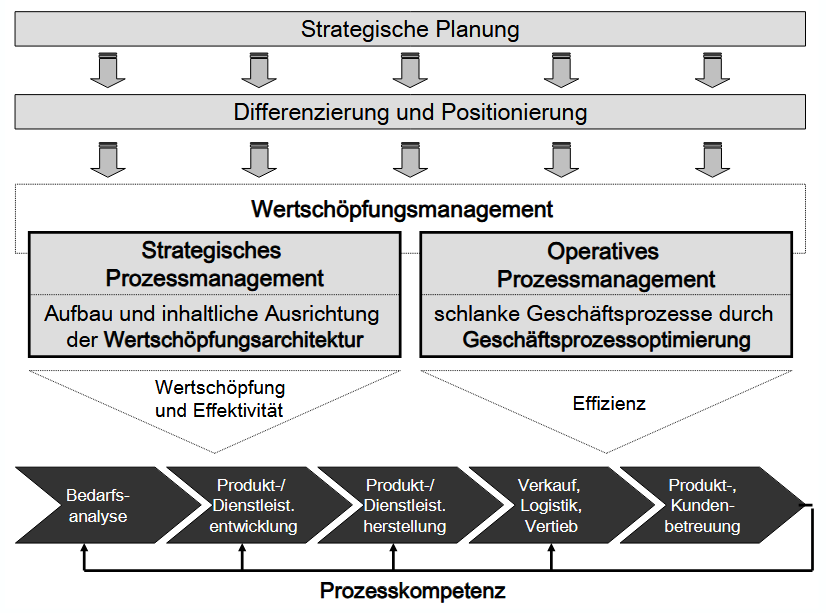
\includegraphics[width=1\linewidth]{./img/wertschöpfungsmanagement}
            \captionof{figure}{wertschöpfungsmanagement}
        \end{center}
        
        \subsection{Wertschöpfungskette}
        \begin{center}
            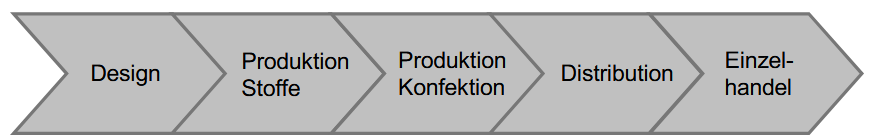
\includegraphics[width=1\linewidth]{./img/wertschöpfungskette}
            \captionof{figure}{wertschöpfungskette}
        \end{center}
        
        \subsection{Wertschöpfungsarchitektur}
        \begin{center}
            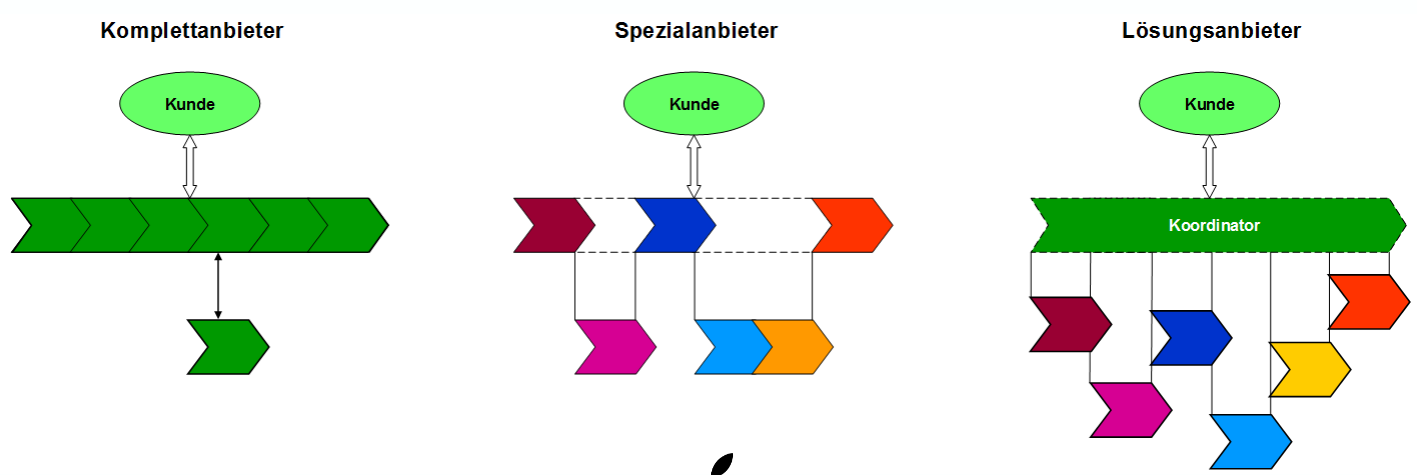
\includegraphics[width=1\linewidth]{./img/wertschöpfungsarchitektur}
            \captionof{figure}{wertschöpfungsarchitektur}
        \end{center}
        
        \subsection{Produktionslogistik}
        
        \begin{itemize}
            \item Produktion = Umwandlung von Gütern/Dienstleistungen.
            \item Produktionslogistik folgt den \textbf{6R}:  
                \begin{quote}
                Richtige Menge – richtiges Objekt – richtiger Ort – richtige Zeit – richtige Qualität – richtige Kosten
                \end{quote}
        \end{itemize}
        
        \subsection{Produktionsprogramm}
        \begin{itemize}
            \item \textbf{Programmbreite}: Anzahl Produktarten
            \item \textbf{Programmtiefe}: Varianten pro Produktart
        \end{itemize}
        \begin{quote}
            Ziel: Gewinnmaximum unter Nebenbedingungen (Kapazität, Absatz, Beschaffung).
        \end{quote}
        
        \subsection{Fertigungsstrategien}
        \begin{itemize}
            \item Fertigungstiefe: gering – mittel – hoch
            \item Make-or-Buy-Entscheid
        \end{itemize}
        
        \subsection{Produktionsplanung und -steuerung (PPS)}
        \begin{center}
            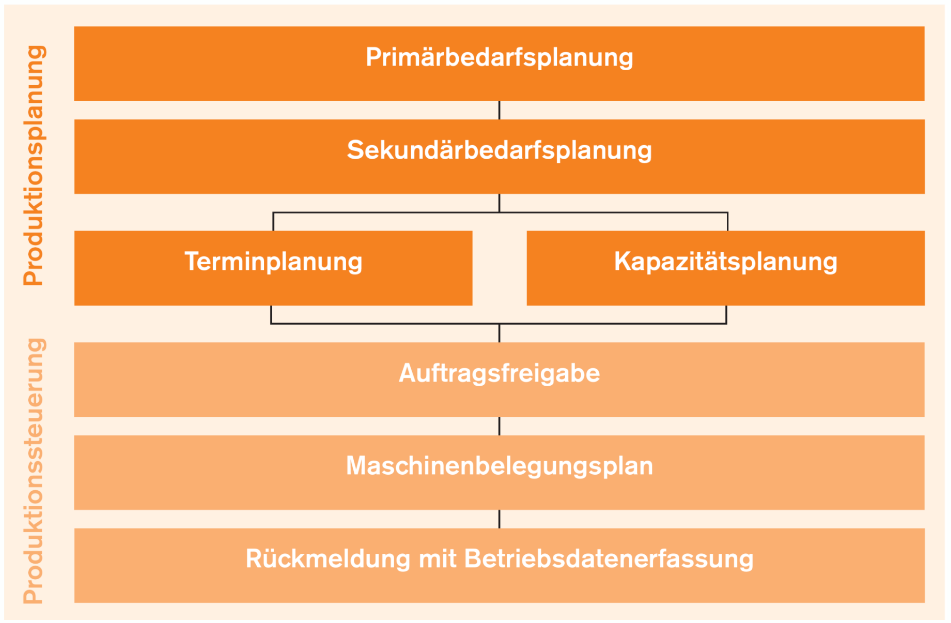
\includegraphics[width=1\linewidth]{./img/produktionsplanung}
            \captionof{figure}{wertschöpfungsarchitektur}
        \end{center}
        
        \subsection{Terminplanung}
        \textbf{Durchlaufzeit}:
        \begin{center}
            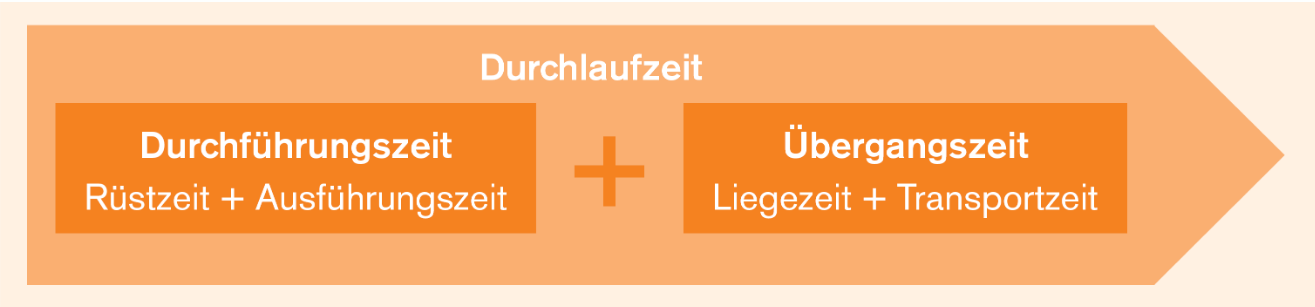
\includegraphics[width=1\linewidth]{./img/durchlaufzeit}
            \captionof{figure}{durchlaufzeit}
        \end{center}
        
        \subsubsection{Terminierung}
        hohe Terminsicherheit, hohe Kapitalbindung
        \textbf{Vorwärtsterminierung}
        \begin{center}
            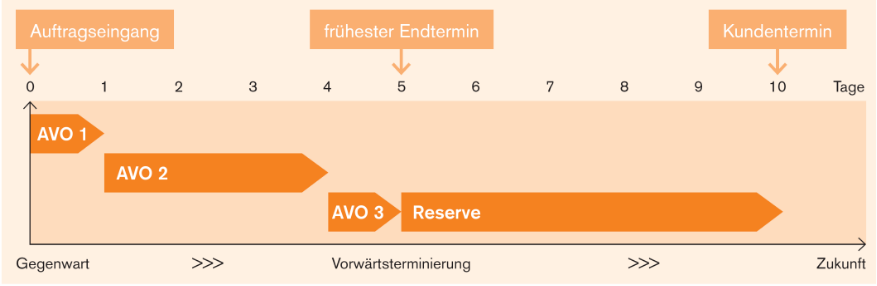
\includegraphics[width=1\linewidth]{./img/vorwärtsterminierung}
            \captionof{figure}{durchlaufzeit}
        \end{center}
        \textbf{Rückwärtsterminierung}
        geringe Lagerkosten, hoher Termindruck
        \begin{center}
            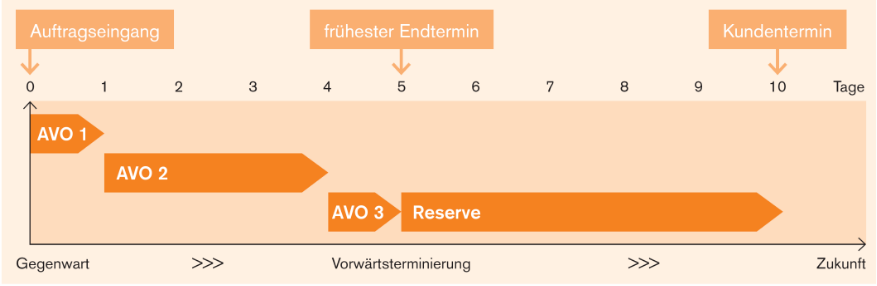
\includegraphics[width=1\linewidth]{./img/rückwärtsterminierung}
            \captionof{figure}{rückwärtsterminierung}
        \end{center}
        
        \section{Nachhaltiges Wirtschaften}
        Nachhaltige Entwicklung:
        \begin{quote}
            Befriedigung heutiger Bedürfnisse ohne Gefährdung zukünftiger Generationen.
        \end{quote}
        
        \subsection{Drei-Säulen-Modell (Triple Bottom Line)}
        \begin{center}
            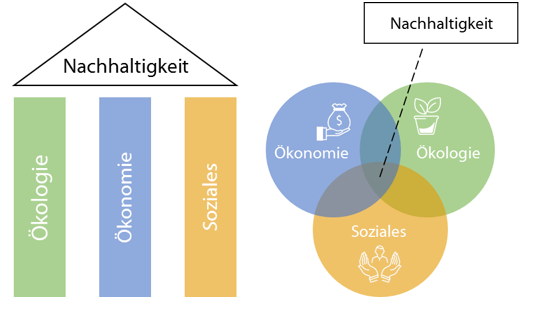
\includegraphics[width=0.6\linewidth]{./img/3säulen}
            \captionof{figure}{3säulen}
        \end{center}
        
        \subsection{Nachhaltigkeitsziele (SDGs)}
        17 globale Ziele der UNO, verpflichtend bis 2030.
        
        \subsection{Verantwortungsbereiche (Scopes)}
        \begin{itemize}
            \item Scope 1: direkte Emissionen
            \item Scope 2: Energiebezug
            \item Scope 3: Lieferkette, Nutzung, Entsorgung
        \end{itemize}
        
        \subsection{Motivation für Unternehmen}
        \begin{itemize}
            \item Wirtschaftlich (Kosteneinsparung, Wettbewerb)
            \item Wertebasiert
            \item Gesetzlich (CSRD, ESRS, Klimagesetz)
        \end{itemize}
        
        \subsection{CSR – Corporate Social Responsibility}
        Freiwillige Verantwortung für Umwelt, Gesellschaft und Unternehmensführung.
        
        \subsection{Greenwashing}
        Täuschende Nachhaltigkeitskommunikation ohne reale Wirkung – Risiko für Reputation und Recht.
        
        
    \end{multicols}
    
    \begin{center}
        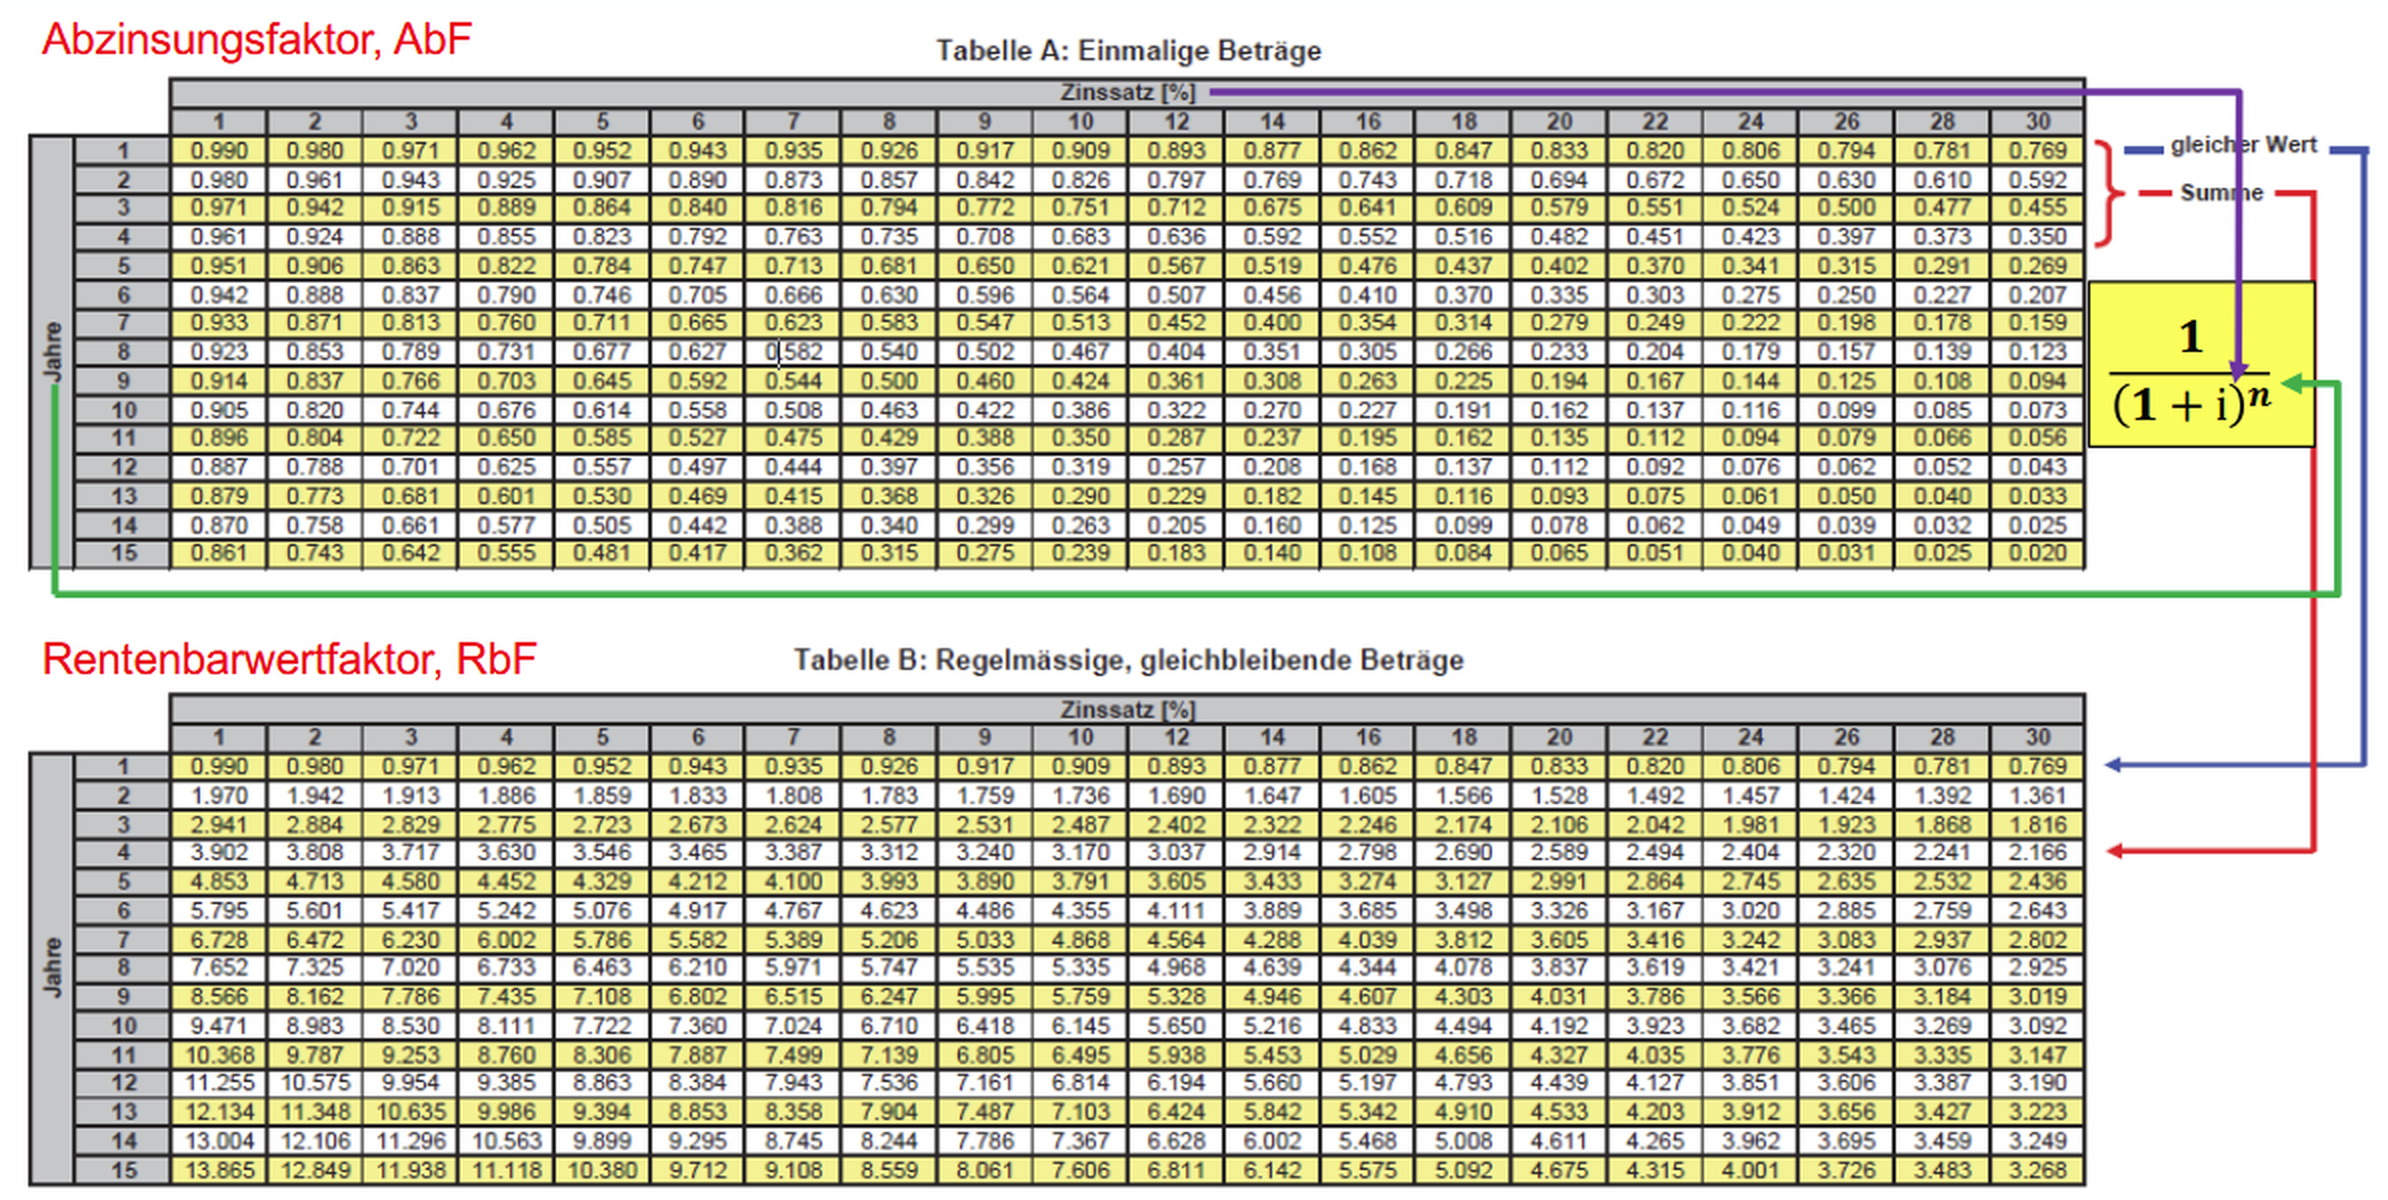
\includegraphics[width=1\linewidth]{./img/zinstabelle}
        \captionof{figure}{zinstabelle}
    \end{center}
    
\end{document}
